\begin{center}
    \section*{\fontsize{20}{20}\selectfont Chapter 4}
\end{center}
\vspace{10mm}

\section{Implementation and Result Analysis}

This chapter presents the practical realization, experimental setup, and comprehensive evaluation of the proposed plant disease detection system. While the preceding chapter outlined the theoretical framework and research methodology, this chapter details the step-by-step execution of the research work, spanning from the development environment setup to the final validation of results.

The main objective of this phase is to test the proposed Custom Lightweight CNN Model by comparing it with two established architectures: ResNet50 and MobileNetV2. The workflow starts with the computational environment, followed by data preprocessing and augmentation of the Potato Leaf Disease Dataset in Uncontrolled Environment. Next, the training process of each model is documented, including the callbacks used (Early Stopping, ReduceLROnPlateau and ModelCheckpoint). The trained models are tested on unseen data and analyzed with Accuracy, Precision, Recall, F1-Score, Confusion Matrices and ROC curves. The chapter also presents the Grad-CAM results and the output of the LLM advisory module. All numbers in this chapter are taken directly from the outputs of the experiment notebook.

\subsection{Environment Setup}
Training deep learning models requires a suitable computational environment. This section describes the software frameworks, programming tools and hardware used to implement, train and test the models.

\subsubsection{Development Environment}
The experimental framework was developed in Python. The deep learning tasks were executed with TensorFlow 2.20.0 as the backend framework and Keras as the high-level API. NumPy 2.0.2 and Pandas were used for data handling, OpenCV and PIL for image processing, Scikit-learn for data splitting and evaluation metrics, and Matplotlib, Seaborn and Plotly for visualization. Random seeds were fixed to 42 for NumPy, TensorFlow and Python to improve reproducibility.

The code was written and run in a Jupyter Notebook on the Kaggle cloud platform. The \texttt{google-genai} library was installed to connect the trained model with the Gemini API. The best model of each run was saved in the native Keras format (\texttt{.keras}) with \texttt{ModelCheckpoint}, so that it could be loaded later for evaluation.

\subsubsection{Hardware and Software Configuration}
Kaggle provides free GPU accelerators. However, the training log of the reported run shows the message ``failed call to cuInit: CUDA error''. This means that the GPU was not available, so all training was done on the CPU. As a result, one epoch of the Custom CNN took about 520 seconds. The configuration is summarized in Table~\ref{tab:hw_sw}.

\begin{table}[htbp]
\caption{Hardware and Software Configuration}
\label{tab:hw_sw}
\begin{center}
\begin{tabularx}{\textwidth}{| p{4.8cm} | X |}
\hline
\textbf{Component} & \textbf{Specification} \\
\hline
Operating System & Linux (Kaggle Notebook kernel) \\
\hline
Platform & Kaggle cloud notebook \\
\hline
GPU (Graphics Processing Unit) & Not active in this run (CUDA initialization failed) \\
\hline
Processor Used & Kaggle cloud CPU \\
\hline
Batch Size / Image Size & $32$ / $224 \times 224 \times 3$ \\
\hline
Programming Language & Python 3 \\
\hline
Deep Learning Framework & TensorFlow 2.20.0, Keras \cite{abadi2016tensorflow} \\
\hline
Key Libraries & NumPy 2.0.2, Pandas, Matplotlib, Seaborn, Scikit-learn, OpenCV, \texttt{google-genai} \\
\hline
\end{tabularx}
\end{center}
\end{table}

\subsection{Data Preprocessing}

\subsubsection{Dataset Description and Class Distribution}
The experiments use the Potato Leaf Disease Dataset in Uncontrolled Environment \cite{shabrina2024novel}. It contains 3,076 color images of potato leaves taken in real fields. The images are grouped into 7 classes: six types of problems (Bacteria, Fungi, Nematode, Pest, Phytopthora and Virus) and one Healthy class.

\textbf{Critical Finding: Class Imbalance.} The dataset is not balanced. As shown in Table~\ref{tab:class_dist}, Fungi is the largest class with 748 images, while Nematode has only 68 images. The ratio between the largest and the smallest class is about 11:1, and the Healthy class is also small (201 images). This imbalance is a challenge for training, because a model can reach a lower loss by favoring the large classes.

\begin{table}[htbp]
\caption{Detailed Class Distribution of the Potato Leaf Disease Dataset}
\label{tab:class_dist}
\begin{center}
\begin{tabularx}{0.85\textwidth}{| X | X | c |}
\hline
\textbf{Plant Name} & \textbf{Disease / Health Status} & \textbf{Number of Images} \\
\hline
Potato & Fungi & 748 \\
\hline
Potato & Pest & 611 \\
\hline
Potato & Bacteria & 569 \\
\hline
Potato & Virus & 532 \\
\hline
Potato & Phytopthora & 347 \\
\hline
Potato & Healthy & 201 \\
\hline
Potato & Nematode & 68 \\
\hline
\textbf{Total Images} & & \textbf{3,076} \\
\hline
\end{tabularx}
\end{center}
\end{table}

\subsubsection{Exploratory Data Analysis (EDA)}
Prior to model training, a comprehensive Exploratory Data Analysis (EDA) was conducted to understand the fundamental characteristics of the Potato Leaf Disease Dataset. This step was crucial for identifying potential biases, understanding image properties, and determining the necessary preprocessing strategies.

\textbf{Visual Inspection of Samples:} Random samples from different classes were visualized to examine the diversity of the dataset. As shown in Figure~\ref{fig:samples}, the images are real field photos. They contain soil, plastic mulch, human hands and neighboring leaves in the background. The symptoms (brown lesions, holes made by pests, yellowing and dark patches) are visible, but they often cover only a small part of the image.

\begin{figure}[htbp]
\centering
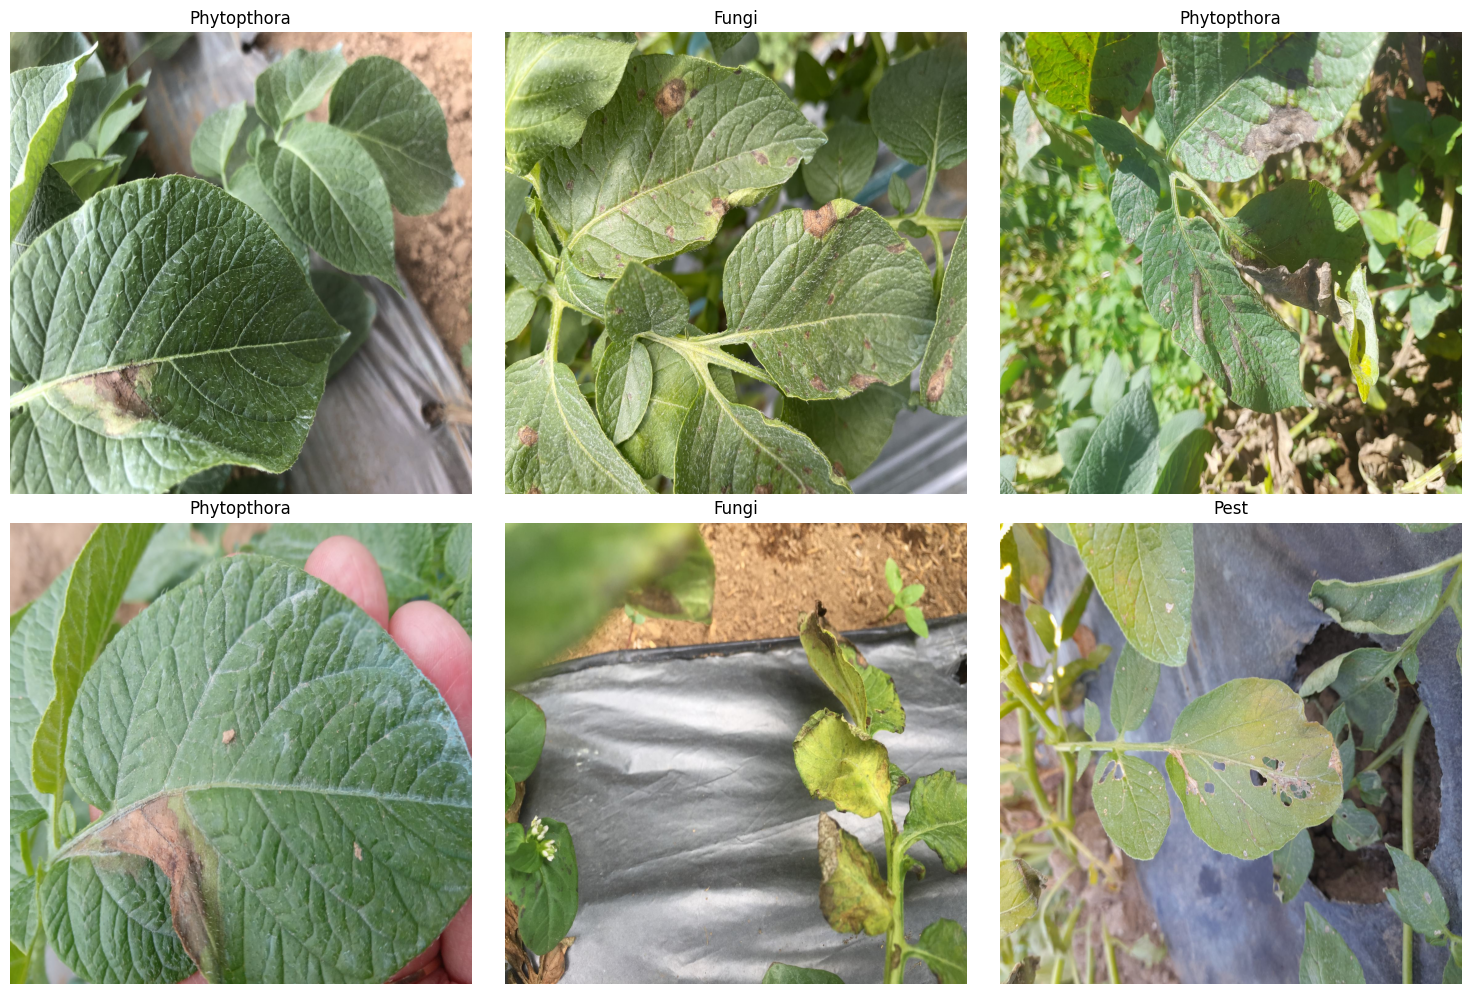
\includegraphics[width=0.9\textwidth]{image/docx_image3.png}
\caption{Sample images from the Potato Leaf Disease Dataset in Uncontrolled Environment.}
\label{fig:samples}
\end{figure}

\textbf{Class Distribution Analysis:} To assess the balance of the dataset, we plotted the frequency of images per class (Figure~\ref{fig:class_dist}). Fungi has the highest number of samples (748), followed by Pest (611), Bacteria (569) and Virus (532). Phytopthora (347), Healthy (201) and especially Nematode (68) are minority classes. This imbalance (about 11:1) creates a risk of model bias toward the majority classes. To reduce this risk, data augmentation was applied during training, and stratified splitting was used so that every class appears in all subsets.

\begin{figure}[htbp]
\centering
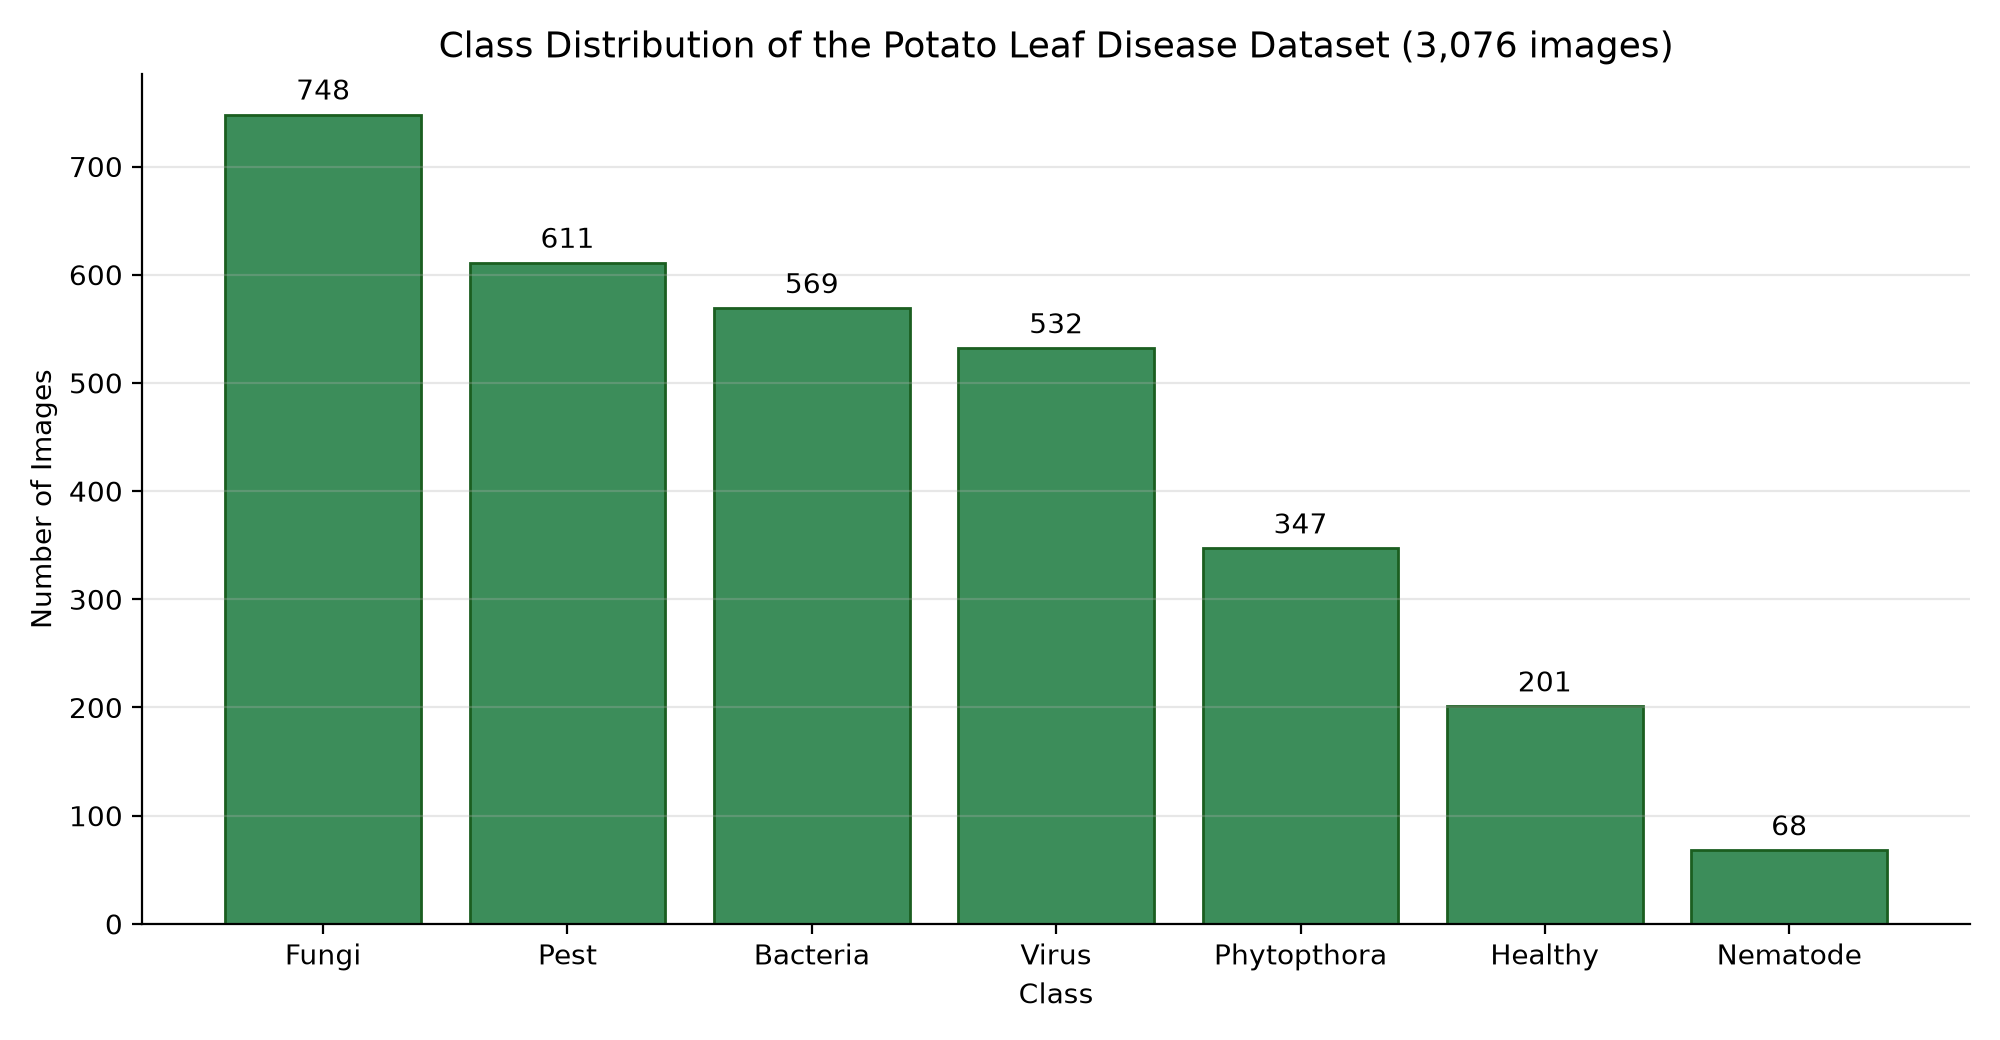
\includegraphics[width=0.85\textwidth]{image/docx_image4.png}
\caption{Class distribution of the Potato Leaf Disease Dataset showing class imbalance.}
\label{fig:class_dist}
\end{figure}

\textbf{Pixel Intensity Analysis:} We analyzed the color properties of the images by computing normalized RGB histograms for 50 randomly selected images. The mean distribution and its confidence band are shown in Figure~\ref{fig:rgb_dist}. The Green channel has the highest intensities, with a peak around 140 to 150, which is expected for leaf images. The Red channel peaks around 100 to 110, and the Blue channel is spread over lower values. A sharp spike at intensity 0 in the Blue channel shows that some images contain very dark regions such as shadows and soil. Unlike laboratory datasets, there is no uniform background, so the model must learn to separate the leaf from a complex scene.

\begin{figure}[htbp]
\centering
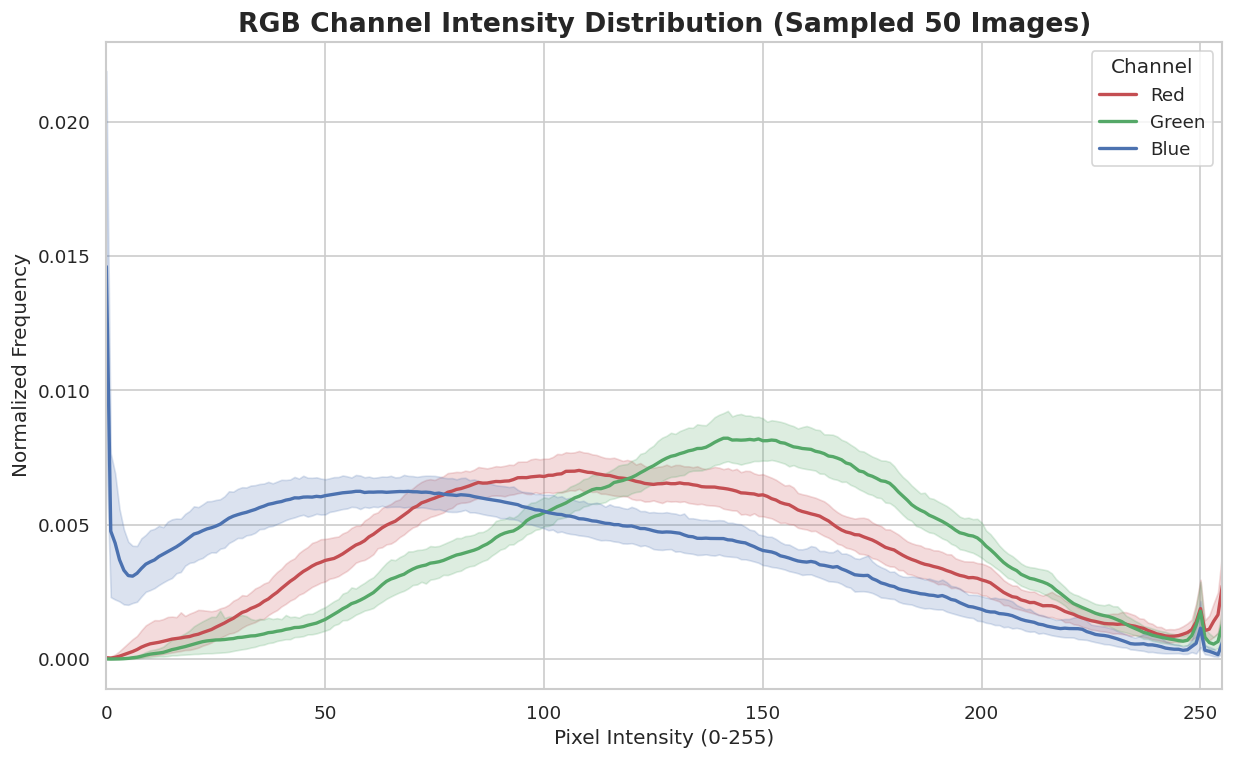
\includegraphics[width=0.85\textwidth]{image/docx_image5.png}
\caption{RGB channel intensity distribution (50 sampled images).}
\label{fig:rgb_dist}
\end{figure}

\subsubsection{Data Splitting Results}
To make the evaluation robust and unbiased, the dataset was divided into three subsets with a ratio of 80:10:10. A stratified strategy (\texttt{random\_state = 42}) was used, so the class proportions are the same in each subset. An integrity check confirmed that all 7 classes are present in the training, validation and test sets (Figure~\ref{fig:data_splits} and Table~\ref{tab:data_splits}):
\begin{itemize}
    \item \textbf{Training Set (80\%):} 2,460 images were used for training. The model uses this subset to learn its weights through backpropagation.
    \item \textbf{Validation Set (10\%):} 308 images were used for validation. This set is used to monitor the model after each epoch, to reduce the learning rate and to trigger Early Stopping.
    \item \textbf{Test Set (10\%):} The remaining 308 images were kept unseen until the final evaluation. It contains 75 Fungi, 61 Pest, 57 Bacteria, 53 Virus, 35 Phytopthora, 20 Healthy and 7 Nematode images.
\end{itemize}

\begin{figure}[htbp]
\centering
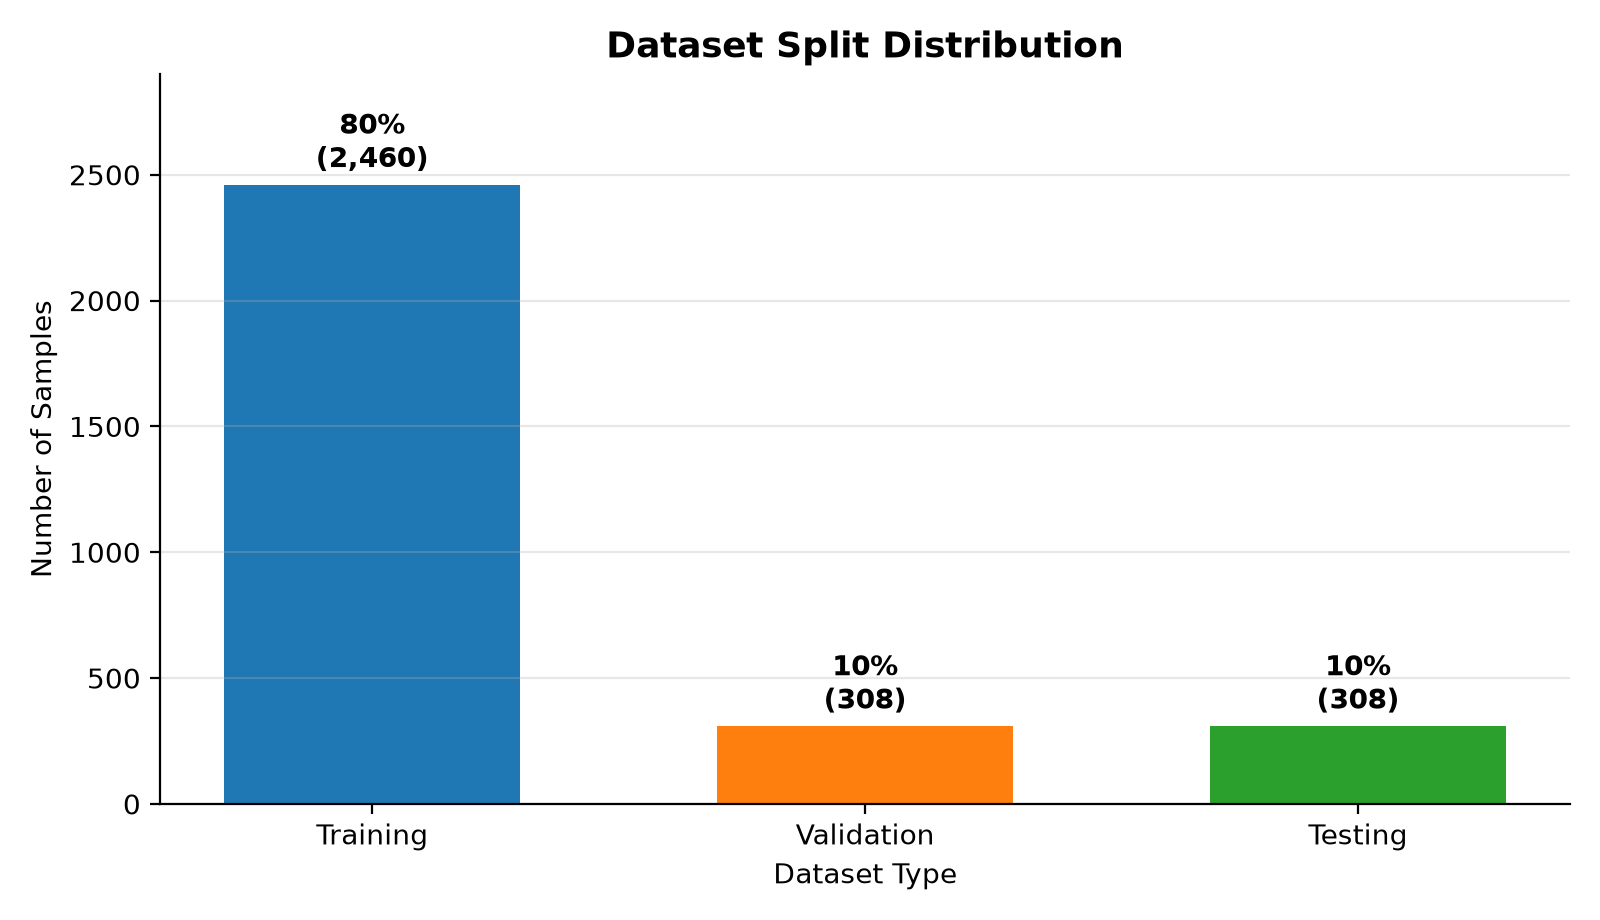
\includegraphics[width=0.85\textwidth]{image/docx_image6.png}
\caption{Data distribution across Training, Validation, and Test sets.}
\label{fig:data_splits}
\end{figure}

\begin{table}[htbp]
\caption{Quantitative Breakdown of Data Splits}
\label{tab:data_splits}
\begin{center}
\begin{tabularx}{0.9\textwidth}{| l | c | c | X |}
\hline
\textbf{Subset} & \textbf{Split Ratio} & \textbf{Image Count} & \textbf{Role in Methodology} \\
\hline
Training & 80\% & 2,460 & Feature Learning \& Weight Update \\
\hline
Validation & 10\% & 308 & Hyperparameter Tuning \& Loss Monitoring \\
\hline
Testing & 10\% & 308 & Final Unbiased Evaluation \\
\hline
\textbf{Total} & \textbf{100\%} & \textbf{3,076} & \\
\hline
\end{tabularx}
\end{center}
\end{table}

\subsubsection{Data Preprocessing and Augmentation Outcomes}
As illustrated in Figure~\ref{fig:preprocess_flow}, our preprocessing pipeline consists of three sequential stages: resizing, normalization tailored to specific model architectures, and on-the-fly data augmentation:
\begin{itemize}
    \item \textbf{Image Resizing:} All images were resized to $224 \times 224$ pixels with 3 color channels (RGB) using the \texttt{target\_size} option of \texttt{flow\_from\_dataframe}.
    \item \textbf{Normalization Strategies (Path A vs.\ Path B):} For the Custom CNN (Path A), pixel values $[0, 255]$ were rescaled to $[0, 1]$ by dividing by $255.0$. For ResNet50 and MobileNetV2 (Path B), the Keras \texttt{preprocess\_input} function of each architecture was used (BGR conversion and ImageNet mean subtraction for ResNet50; scaling to $[-1, 1]$ for MobileNetV2).
    \item \textbf{Data Augmentation Results:} On-the-fly data augmentation was applied to the training set with \texttt{ImageDataGenerator} using random rotation (up to $20^\circ$), width and height shifts (up to 20\%), zoom (up to 20\%, nearest-pixel fill), and horizontal flips.
\end{itemize}

\begin{figure}[htbp]
\centering
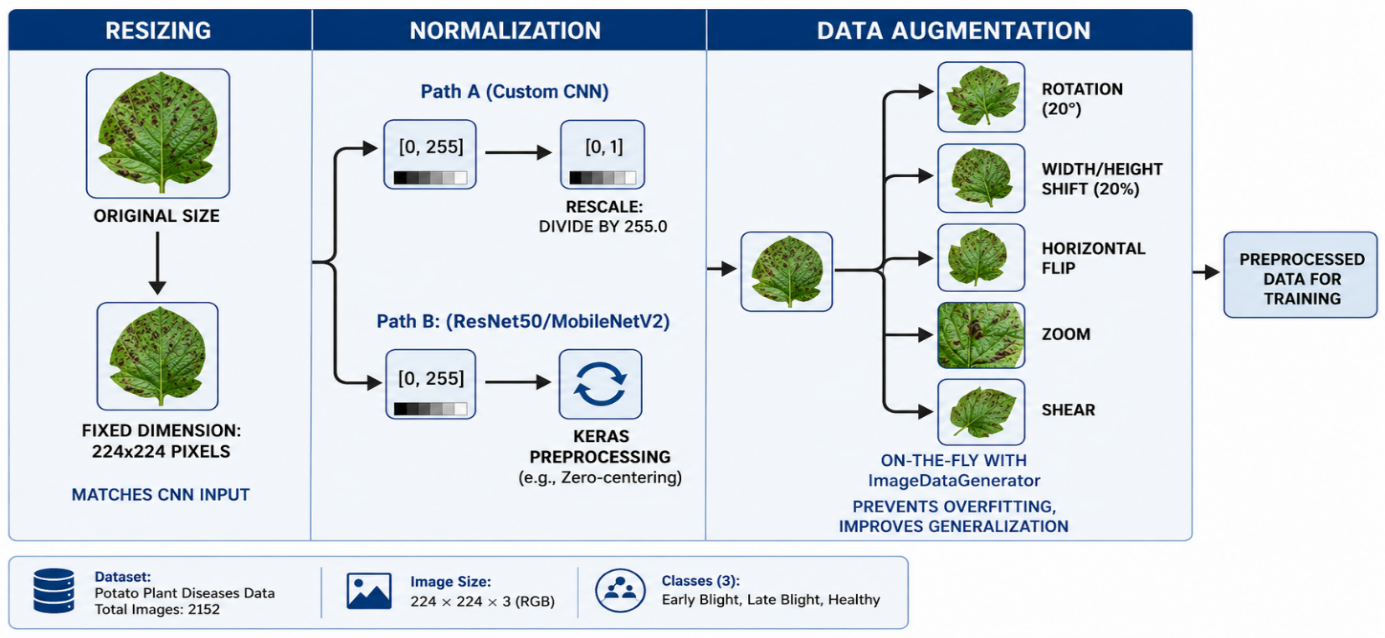
\includegraphics[width=0.9\textwidth]{image/docx_image7.png}
\caption{Data preprocessing workflow illustrating resizing, model-specific normalization (Path A vs.\ Path B), and augmentation.}
\label{fig:preprocess_flow}
\end{figure}

\subsection{Model Implementation}

\subsubsection{Custom CNN (Proposed Model)}
The proposed model is a custom-designed, lightweight Convolutional Neural Network (CNN) tailored for the efficient classification of plant diseases. The architectural flow is visualized in Figure~\ref{fig:custom_cnn_arch}. As detailed in Table~\ref{tab:custom_cnn_layers}, the model uses \texttt{GlobalAveragePooling2D} and Swish activation. It has only 162,887 parameters (636.28 KB of weights), which is much lighter than the other two models.

\begin{figure}[htbp]
\centering
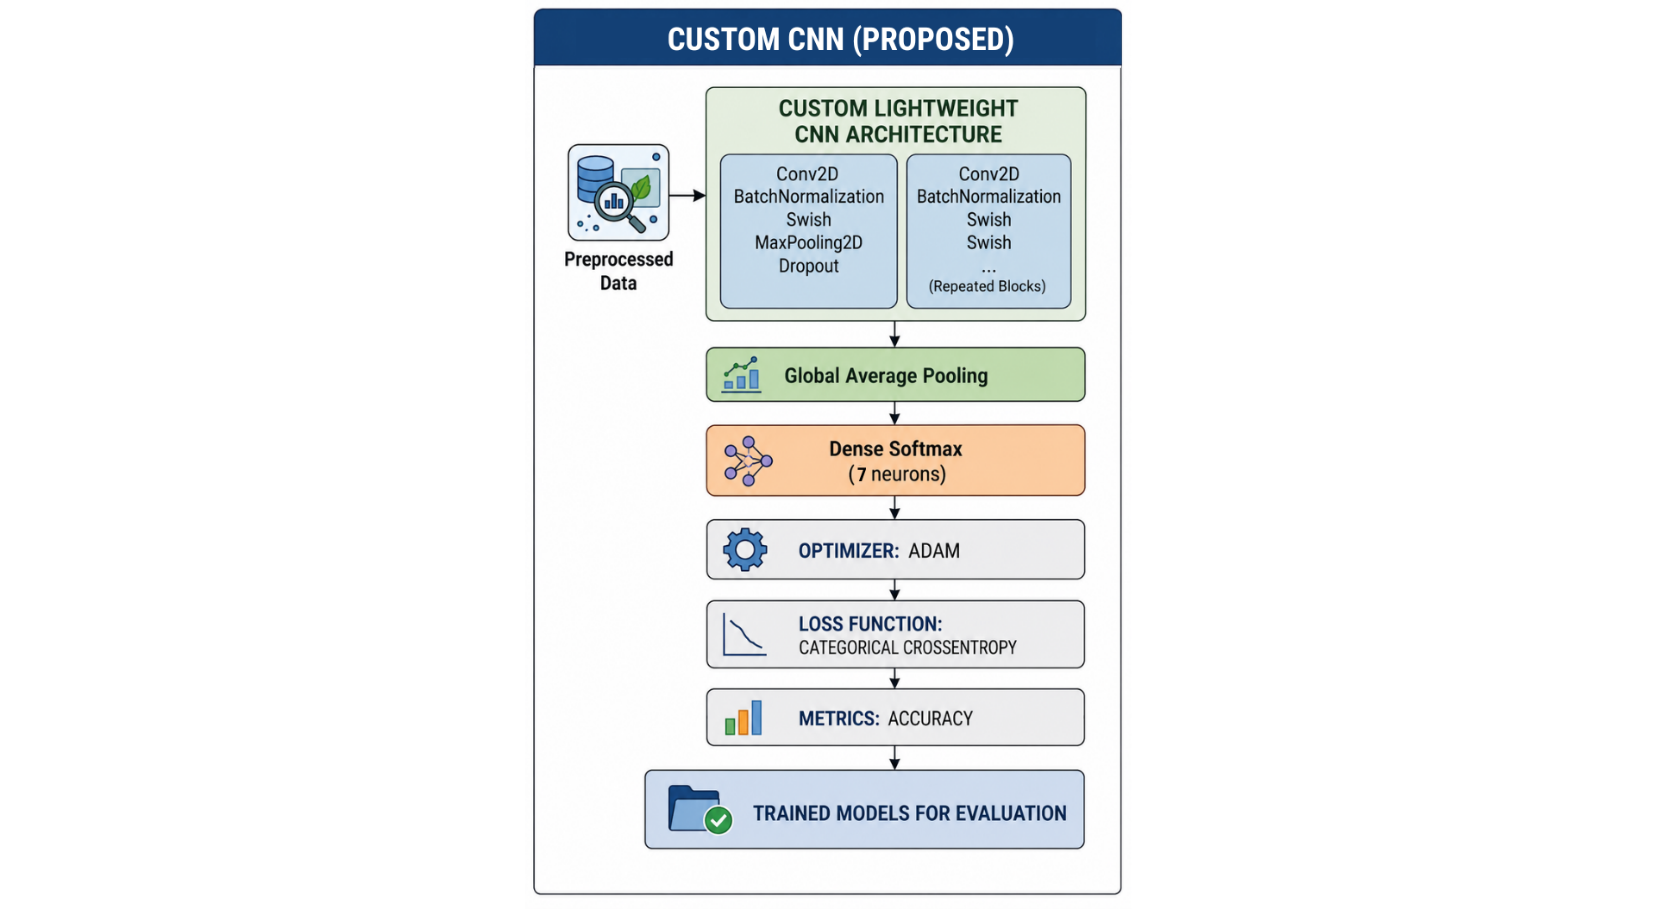
\includegraphics[width=0.9\textwidth]{image/docx_image8.png}
\caption{Architectural design of the proposed Custom Lightweight CNN.}
\label{fig:custom_cnn_arch}
\end{figure}

\begin{table}[htbp]
\caption{Detailed Layer Configuration and Parameter Summary of the Proposed Custom CNN}
\label{tab:custom_cnn_layers}
\begin{center}
\begin{tabularx}{\textwidth}{| X | c | r | X |}
\hline
\textbf{Layer Type} & \textbf{Output Shape} & \textbf{Param \#} & \textbf{Description / Block} \\
\hline
Input Layer & $(224, 224, 3)$ & 0 & Input Image ($224 \times 224$ RGB) \\
\hline
Conv2D (16 filters) & $(224, 224, 16)$ & 448 & Block 1 (Low-Level) \\
\hline
BatchNormalization + Swish & $(224, 224, 16)$ & 64 & Feature Extraction \\
\hline
Conv2D (32 filters) & $(224, 224, 32)$ & 4,640 & \\
\hline
BatchNormalization + Swish & $(224, 224, 32)$ & 128 & \\
\hline
MaxPooling2D + Dropout (0.20) & $(112, 112, 32)$ & 0 & Dimensionality Reduction \\
\hline
Conv2D (32 filters) & $(112, 112, 32)$ & 9,248 & Block 2 (Mid-Level) \\
\hline
BatchNormalization + Swish & $(112, 112, 32)$ & 128 & Feature Extraction \\
\hline
Conv2D (64 filters) & $(112, 112, 64)$ & 18,496 & \\
\hline
BatchNormalization + Swish & $(112, 112, 64)$ & 256 & \\
\hline
MaxPooling2D + Dropout (0.20) & $(56, 56, 64)$ & 0 & Dimensionality Reduction \\
\hline
Conv2D (64 filters) & $(56, 56, 64)$ & 36,928 & Block 3 (High-Level) \\
\hline
BatchNormalization + Swish & $(56, 56, 64)$ & 256 & Feature Extraction \\
\hline
Conv2D (128 filters) & $(56, 56, 128)$ & 73,856 & \\
\hline
BatchNormalization + Swish & $(56, 56, 128)$ & 512 & \\
\hline
MaxPooling2D + Dropout (0.25) & $(28, 28, 128)$ & 0 & Dimensionality Reduction \\
\hline
GlobalAveragePooling2D & $(128)$ & 0 & Classification Head \\
\hline
Dense & $(128)$ & 16,512 & Fully Connected Layer \\
\hline
BatchNormalization + Swish & $(128)$ & 512 & \\
\hline
Dropout (0.40) & $(128)$ & 0 & Regularization \\
\hline
Dense (Output) & $(7)$ & 903 & Softmax Classification (7 Classes) \\
\hline
\textbf{Total Parameters} & & \textbf{162,887} & ($\sim 0.16$ Million, 636.28 KB) \\
\hline
Trainable Parameters & & 161,959 & \\
\hline
Non-trainable Parameters & & 928 & \\
\hline
\end{tabularx}
\end{center}
\end{table}

\subsubsection{ResNet50 (Frozen Backbone)}
ResNet50 was implemented as a deep benchmark model. The base network was loaded without its top classification layers (\texttt{include\_top = False}). Because pre-trained ImageNet weights could not be downloaded in the Kaggle session, the base was created with random weights (\texttt{weights = None}) and then frozen (\texttt{trainable = False}). As illustrated in Figure~\ref{fig:resnet_arch}, a custom classification head (\texttt{GlobalAveragePooling2D}, \texttt{Dense(64)}, \texttt{BatchNormalization}, Swish, \texttt{Dropout(0.3)}, and \texttt{Dense(7)} Softmax) was attached. As summarized in Table~\ref{tab:resnet_params}, the total parameter count is 23,719,559 (90.48 MB), with only 131,719 trainable parameters in the head.

\begin{figure}[htbp]
\centering
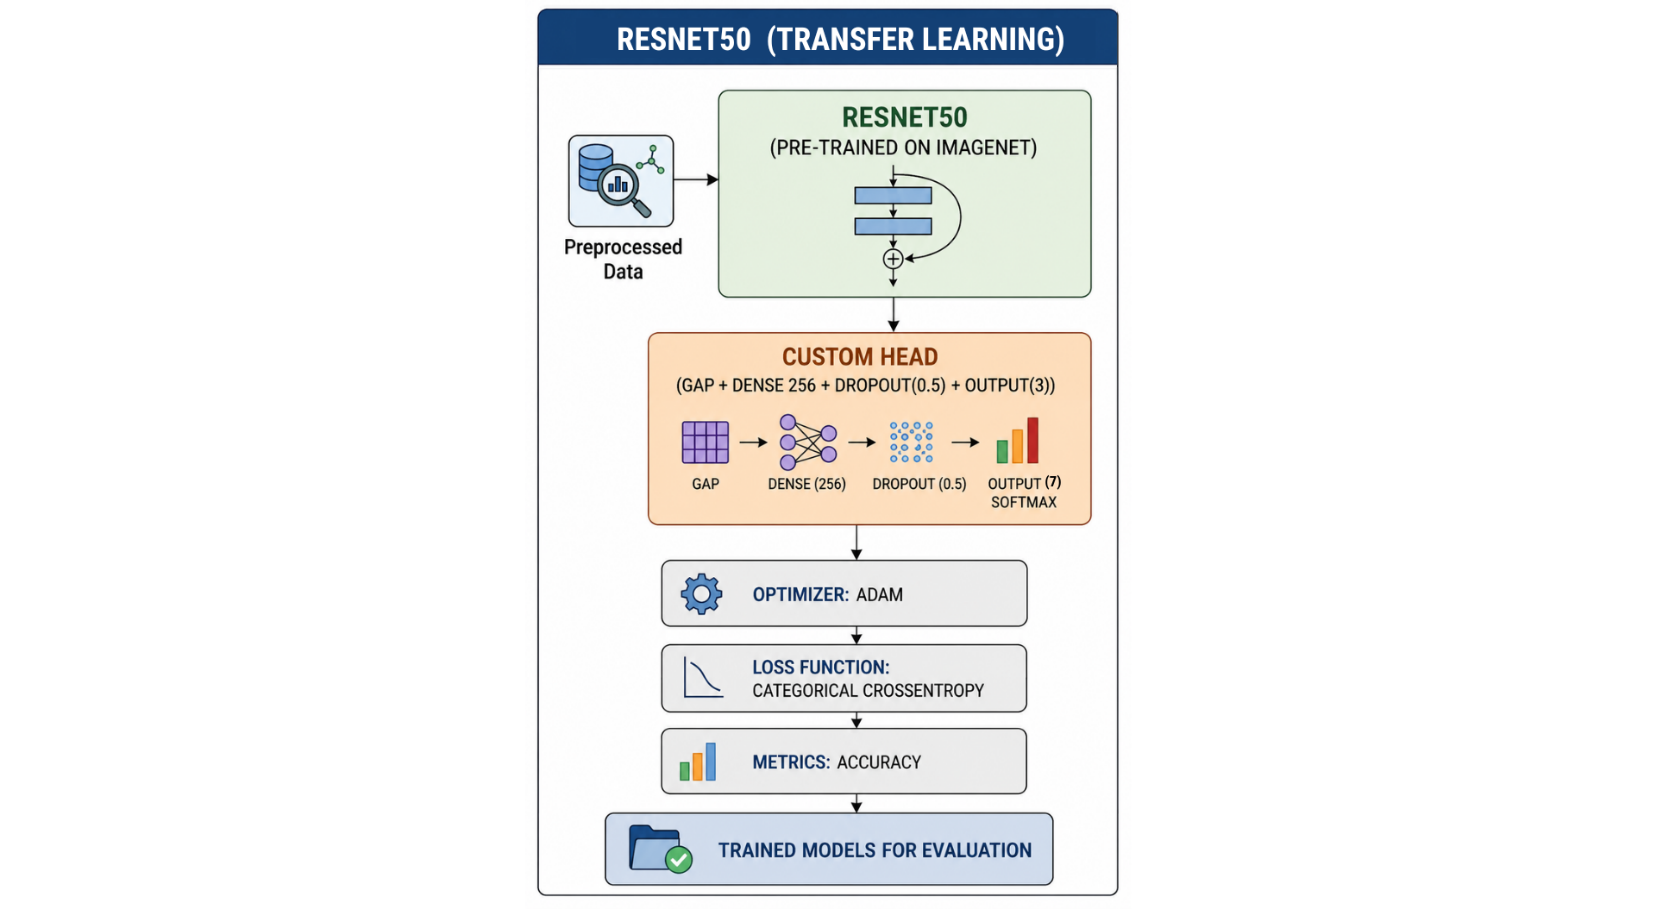
\includegraphics[width=0.9\textwidth]{image/docx_image12.png}
\caption{ResNet50 architecture with the custom classification head.}
\label{fig:resnet_arch}
\end{figure}

\begin{table}[htbp]
\caption{Parameter Summary of ResNet50 Model}
\label{tab:resnet_params}
\begin{center}
\begin{tabularx}{\textwidth}{| l | l | X |}
\hline
\textbf{Parameter Type} & \textbf{Count} & \textbf{Implication} \\
\hline
Total Parameters & 23,719,559 (90.48 MB) & Deep architecture capacity. \\
\hline
Trainable Parameters & 131,719 & Only the custom head is trained. \\
\hline
Non-trainable Parameters & 23,587,840 & Frozen, randomly initialized base. \\
\hline
\end{tabularx}
\end{center}
\end{table}

\subsubsection{MobileNetV2 (Trained from Scratch)}
MobileNetV2 utilizes Depthwise Separable Convolutions to reduce computational complexity. As shown in Figure~\ref{fig:mobilenet_arch}, the MobileNetV2 base (\texttt{include\_top = False}) is followed by the same classification head as ResNet50. Because no pre-trained weights were loaded (\texttt{weights = None}), all layers were set as trainable. As shown in Table~\ref{tab:mobilenet_params}, the model has 2,340,679 total parameters ($\sim 2.34$ million, 8.93 MB), roughly 10 times fewer than ResNet50.

\begin{figure}[htbp]
\centering
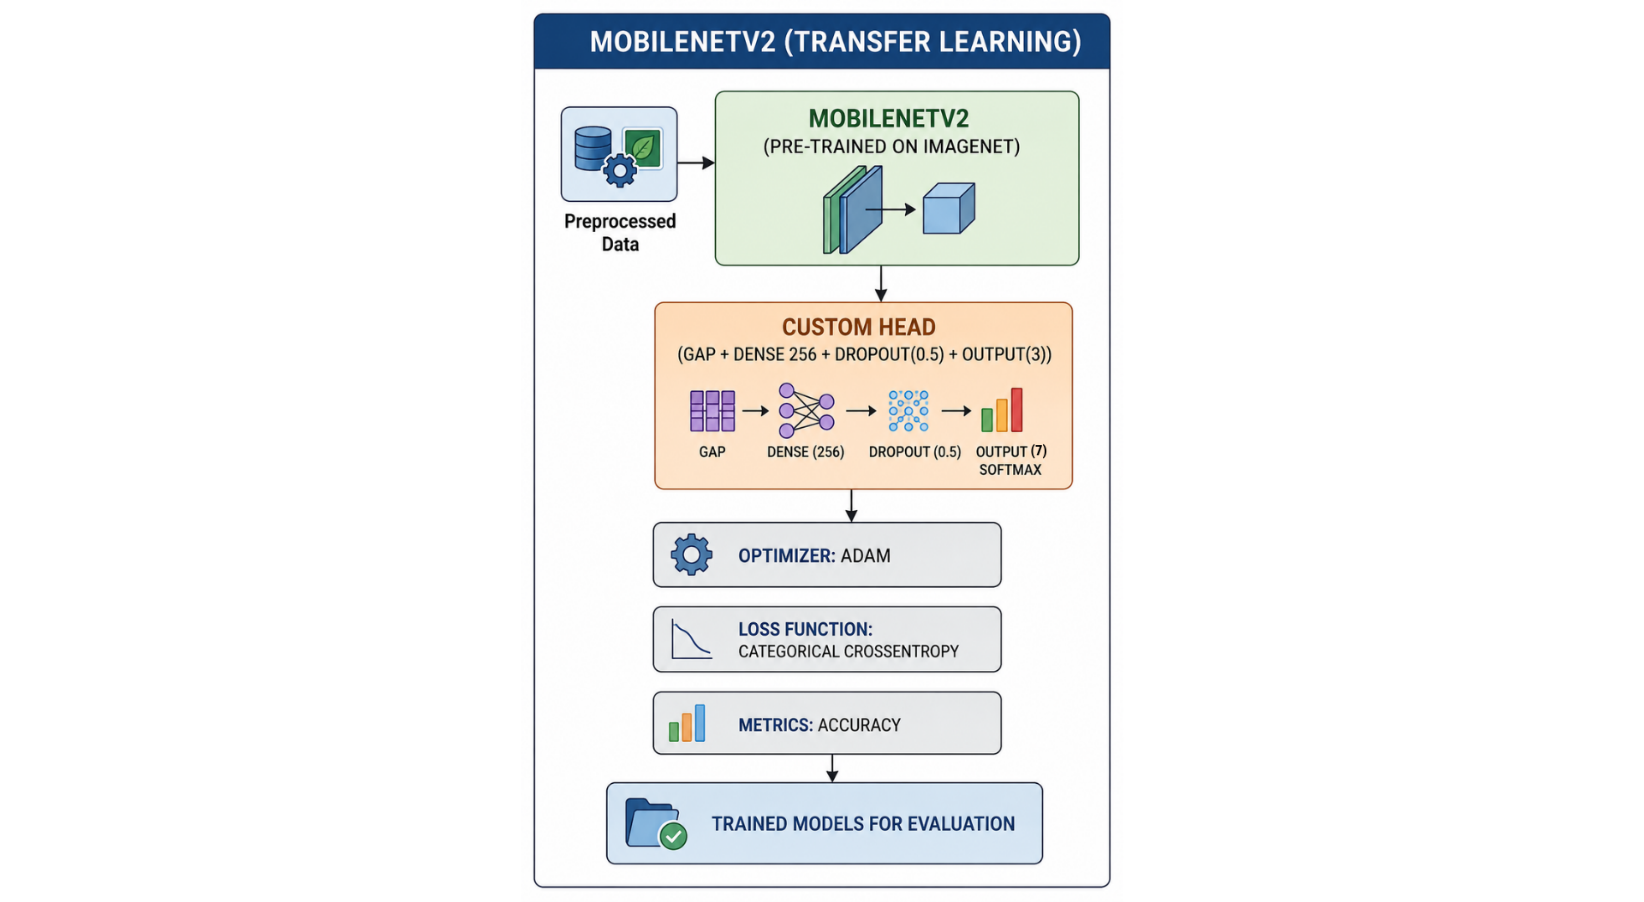
\includegraphics[width=0.9\textwidth]{image/docx_image16.png}
\caption{MobileNetV2 architecture with the custom classification head.}
\label{fig:mobilenet_arch}
\end{figure}

\begin{table}[htbp]
\caption{Model Configuration and Parameter Summary of MobileNetV2}
\label{tab:mobilenet_params}
\begin{center}
\begin{tabularx}{\textwidth}{| p{4.5cm} | X |}
\hline
\textbf{Model Component} & \textbf{Specification / Count} \\
\hline
Base Model & MobileNetV2 (\texttt{weights = None}, random initialization) \\
\hline
Input Shape & $(224, 224, 3)$ \\
\hline
Feature Extractor Status & Trainable (all layers) \\
\hline
Custom Head Layers & GAP $\rightarrow$ Dense(64) $\rightarrow$ BN $\rightarrow$ Swish $\rightarrow$ Dropout(0.3) $\rightarrow$ Softmax(7) \\
\hline
Total Parameters & 2,340,679 ($\sim 2.34$ Million, 8.93 MB) \\
\hline
Trainable Parameters & 2,306,439 \\
\hline
Non-trainable Parameters & 34,240 (Batch Normalization statistics) \\
\hline
\end{tabularx}
\end{center}
\end{table}

\subsection{Evaluation Metrics}
All models were compiled with the Adam optimizer (initial learning rate $0.001$) and Categorical Crossentropy loss with label smoothing ($0.1$). Performance on the 308 unseen test images was evaluated using Accuracy, Test Loss, Precision, Recall, F1-Score, Confusion Matrices, micro-average ROC-AUC, inference latency (ms/image on CPU), and saved model size (MB).

\subsection{Performance Analysis}

\subsubsection{Custom CNN Results}
The Custom CNN was set to train for 15 epochs with a batch size of 32 (77 steps per epoch). Early Stopping (patience 5) stopped training after Epoch 6 because validation loss did not improve after Epoch 1 (best validation loss $1.9509$ at Epoch 1 vs.\ $2.1902$ at Epoch 6), and \texttt{ReduceLROnPlateau} reduced the learning rate from $0.001$ to $0.0002$ after Epoch 4. Training accuracy rose from 33.17\% (Epoch 1) to 50.20\% (Epoch 6), while validation accuracy stayed between 19.81\% and 35.71\% (Figure~\ref{fig:cnn_curves}).

\begin{figure}[htbp]
\centering
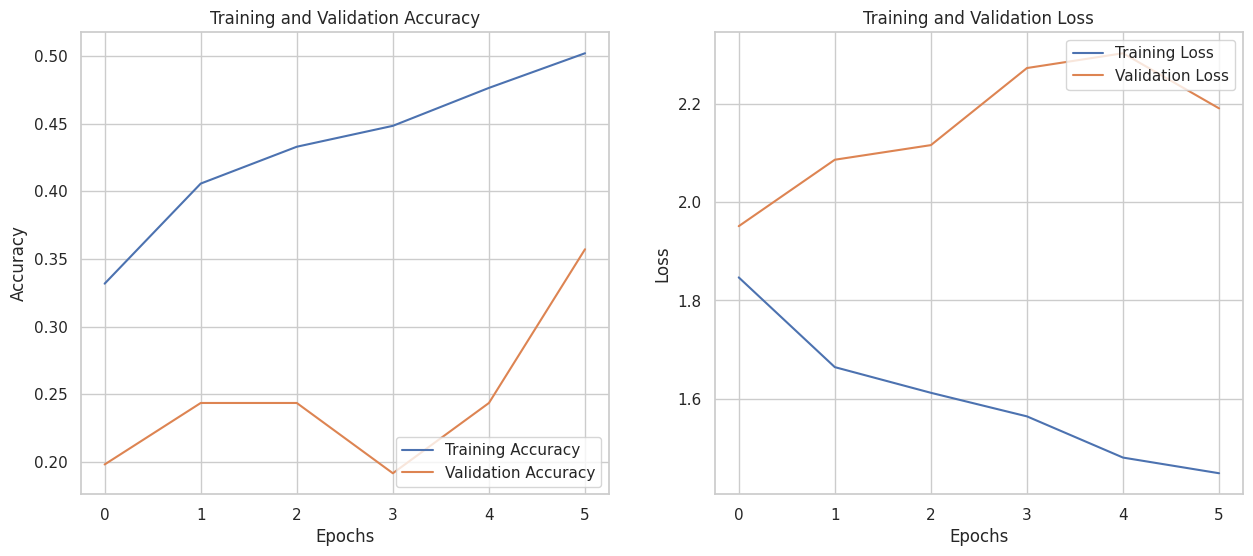
\includegraphics[width=0.9\textwidth]{image/docx_image9.png}
\caption{Training and validation accuracy/loss curves of the Custom CNN.}
\label{fig:cnn_curves}
\end{figure}

On the 308 unseen test images, the restored Epoch 1 checkpoint achieved a Test Accuracy of 19.81\% and a Test Loss of 1.9508 (Table~\ref{tab:cnn_report}). The model predicted \textbf{Pest} for all 308 test images (recall $1.00$, precision $0.20$, F1-score $0.33$), while the remaining six classes scored $0.00$ across precision, recall, and F1-score. This single-class collapse is confirmed by the confusion matrix (Figure~\ref{fig:cnn_cm}) and the random sample predictions (Figure~\ref{fig:cnn_samples}), where every sample is predicted as Pest with $\sim 21\%$ confidence.

\begin{table}[htbp]
\caption{Summary of Classification Report (Custom CNN)}
\label{tab:cnn_report}
\begin{center}
\begin{tabularx}{0.65\textwidth}{| X | c |}
\hline
\textbf{Metric} & \textbf{Score} \\
\hline
Accuracy & 19.81\% \\
\hline
Macro Average (Precision) & 0.03 \\
\hline
Macro Average (Recall) & 0.14 \\
\hline
Macro Average (F1-Score) & 0.05 \\
\hline
Weighted Average F1-Score & 0.07 \\
\hline
\end{tabularx}
\end{center}
\end{table}

\begin{figure}[htbp]
\centering
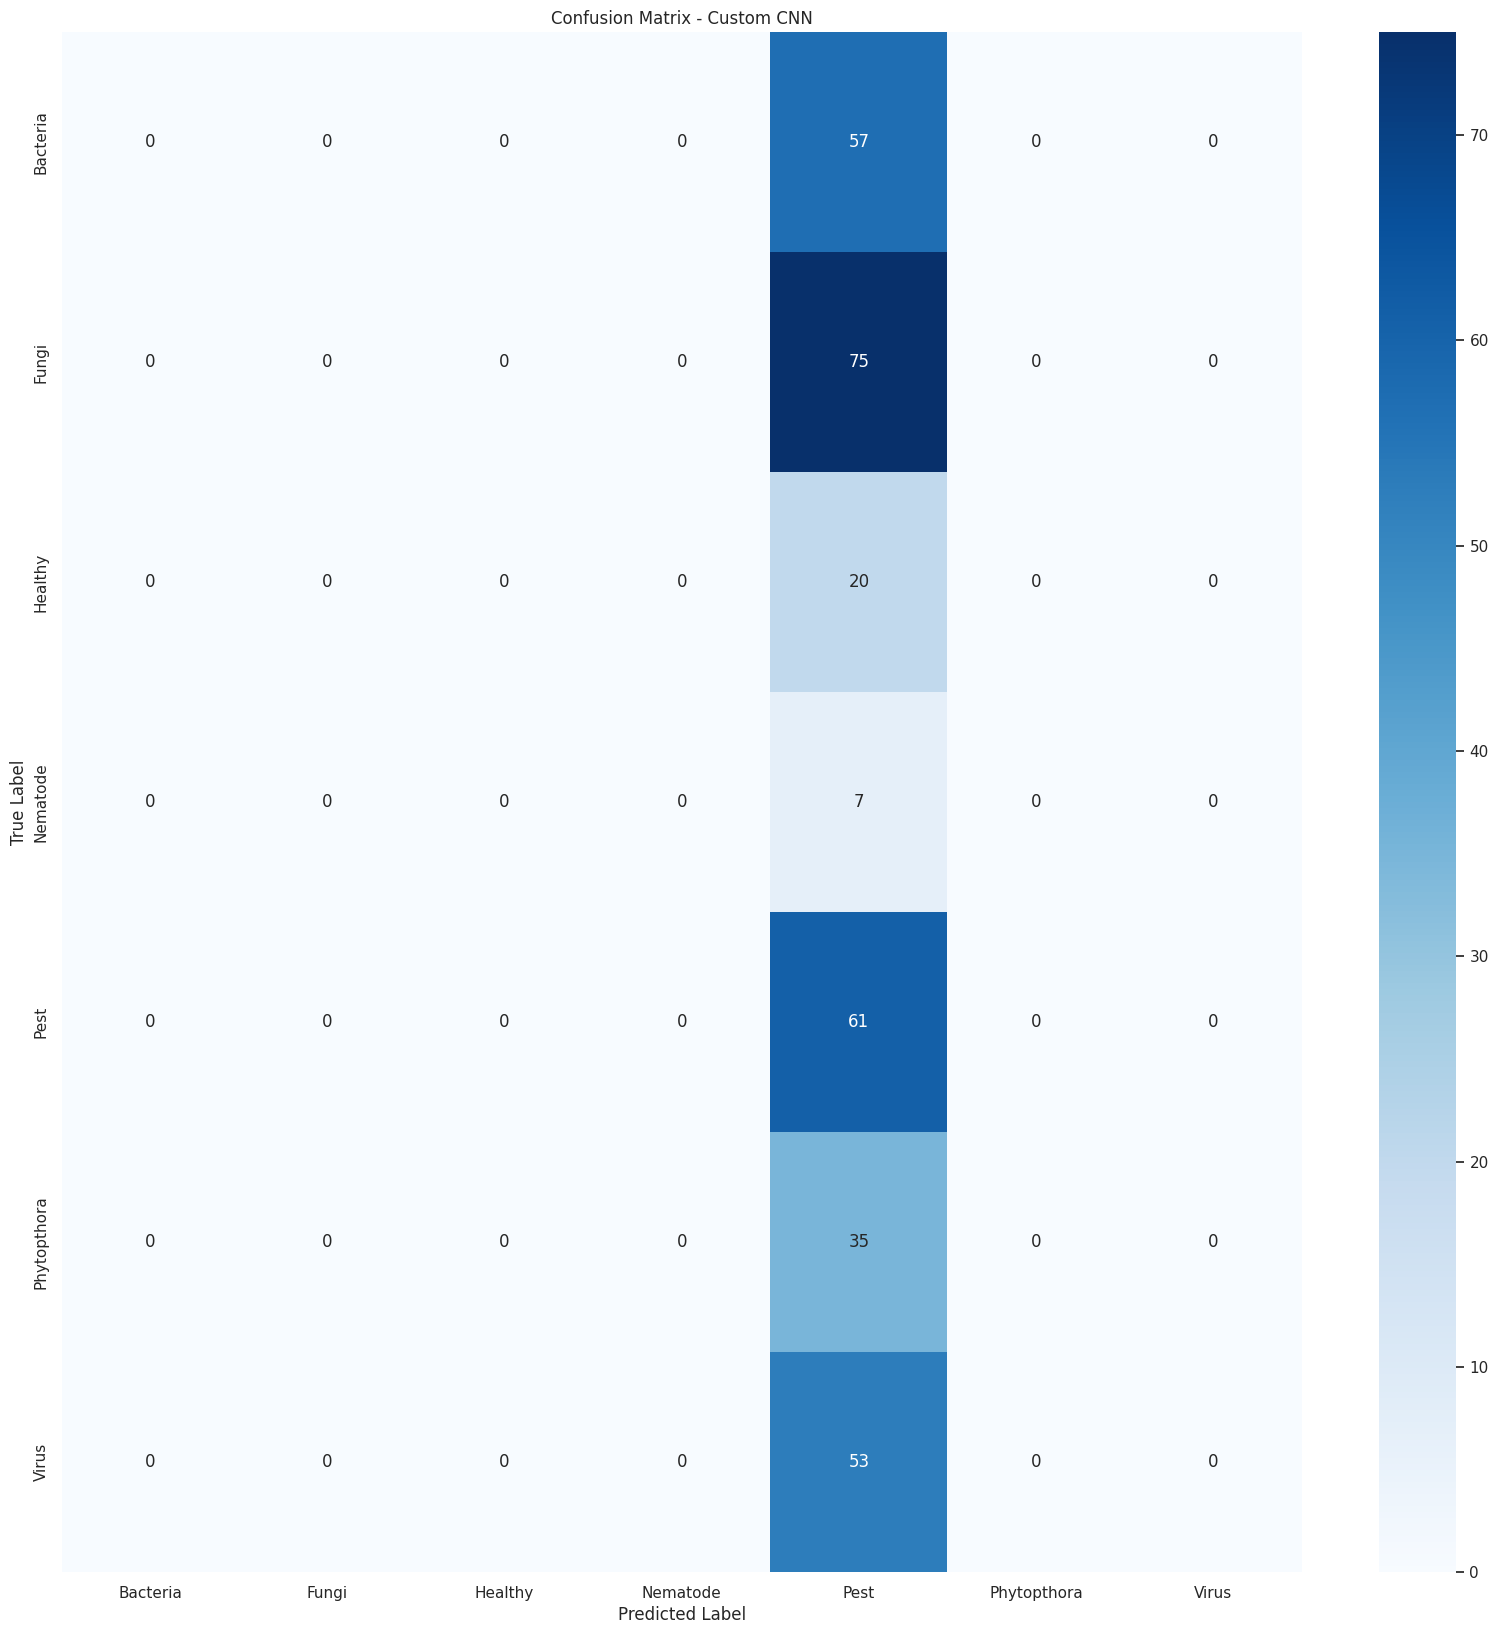
\includegraphics[width=0.75\textwidth]{image/docx_image10.png}
\caption{Confusion Matrix for Custom CNN on the test set.}
\label{fig:cnn_cm}
\end{figure}

\begin{figure}[htbp]
\centering
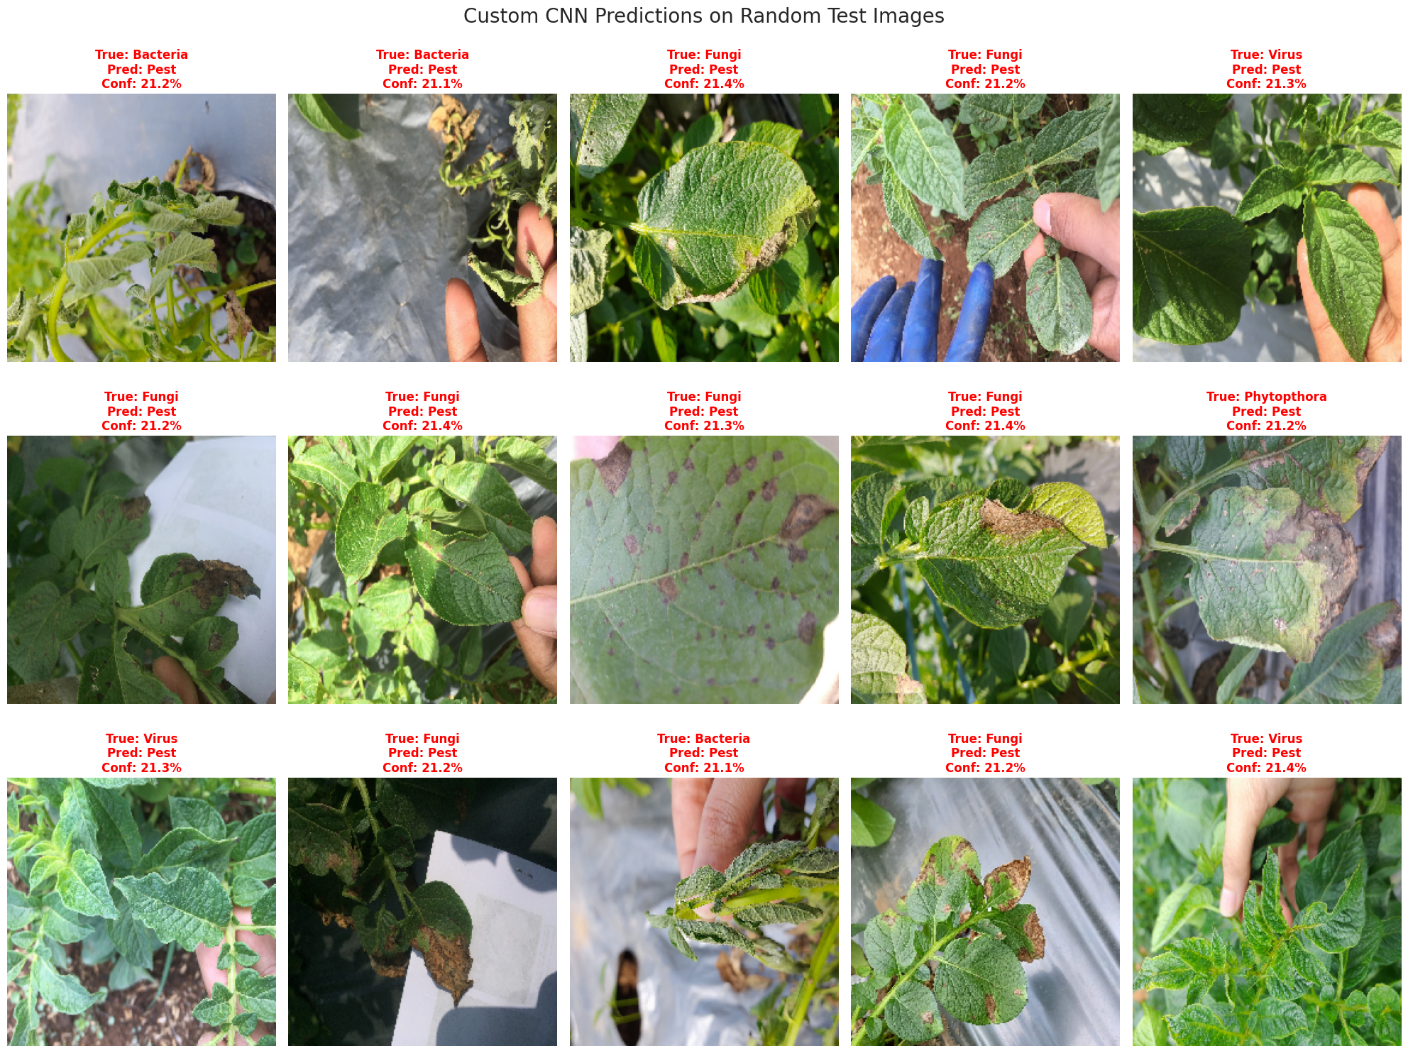
\includegraphics[width=0.9\textwidth]{image/docx_image11.png}
\caption{Random test samples predicted by the Custom CNN (red titles are wrong predictions).}
\label{fig:cnn_samples}
\end{figure}

\subsubsection{ResNet50 Results}
ResNet50 was trained for 10 epochs ($\sim 245$ seconds per epoch on CPU), with the learning rate reduced to $0.0002$ after Epoch 8. Epoch 10 achieved the lowest validation loss ($1.7539$) with 42.97\% training accuracy and 30.19\% validation accuracy (Figure~\ref{fig:resnet_curves}).

\begin{figure}[htbp]
\centering
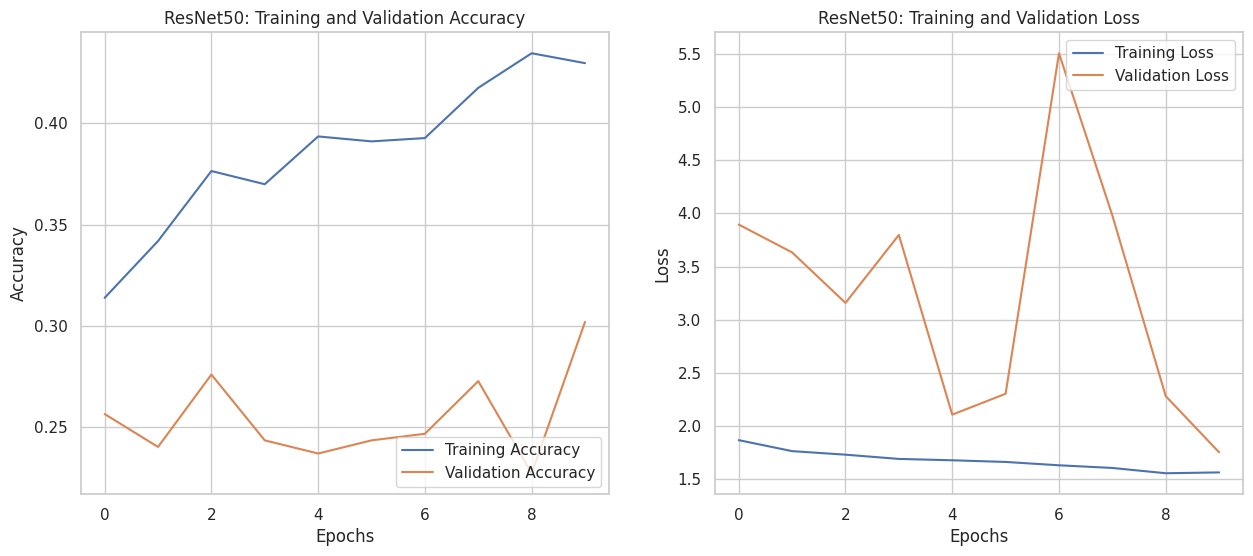
\includegraphics[width=0.9\textwidth]{image/docx_image13.png}
\caption{Training and validation accuracy/loss curves for ResNet50.}
\label{fig:resnet_curves}
\end{figure}

On the 308 test images, ResNet50 achieved a Test Accuracy of 31.82\% and a Test Loss of 1.7336 (Table~\ref{tab:resnet_report}), the highest of the three models. Virus achieved the best F1-score (0.54; precision 0.76, recall 0.42), and Nematode had precision 1.00 (recall 0.29, 2 of 7 images). Pest had high recall (0.77) but low precision (0.22), while Healthy had F1-score 0.00 and Bacteria/Phytopthora had recalls of 0.04 and 0.09. As shown in Figure~\ref{fig:resnet_cm}, 98 of 308 images lie on the diagonal, though 47 Bacteria and 52 Fungi images were misclassified as Pest. In the random sample visualization (Figure~\ref{fig:resnet_samples}), 6 of 15 images are correct, with confidences ranging from 30\% to 77\%.

\begin{table}[htbp]
\caption{Summary of Classification Report (ResNet50)}
\label{tab:resnet_report}
\begin{center}
\begin{tabularx}{0.65\textwidth}{| X | c |}
\hline
\textbf{Metric} & \textbf{Score} \\
\hline
Accuracy & 31.82\% \\
\hline
Macro Avg (Precision) & 0.52 \\
\hline
Macro Avg (Recall) & 0.27 \\
\hline
Weighted Avg F1-Score & 0.28 \\
\hline
\end{tabularx}
\end{center}
\end{table}

\begin{figure}[htbp]
\centering
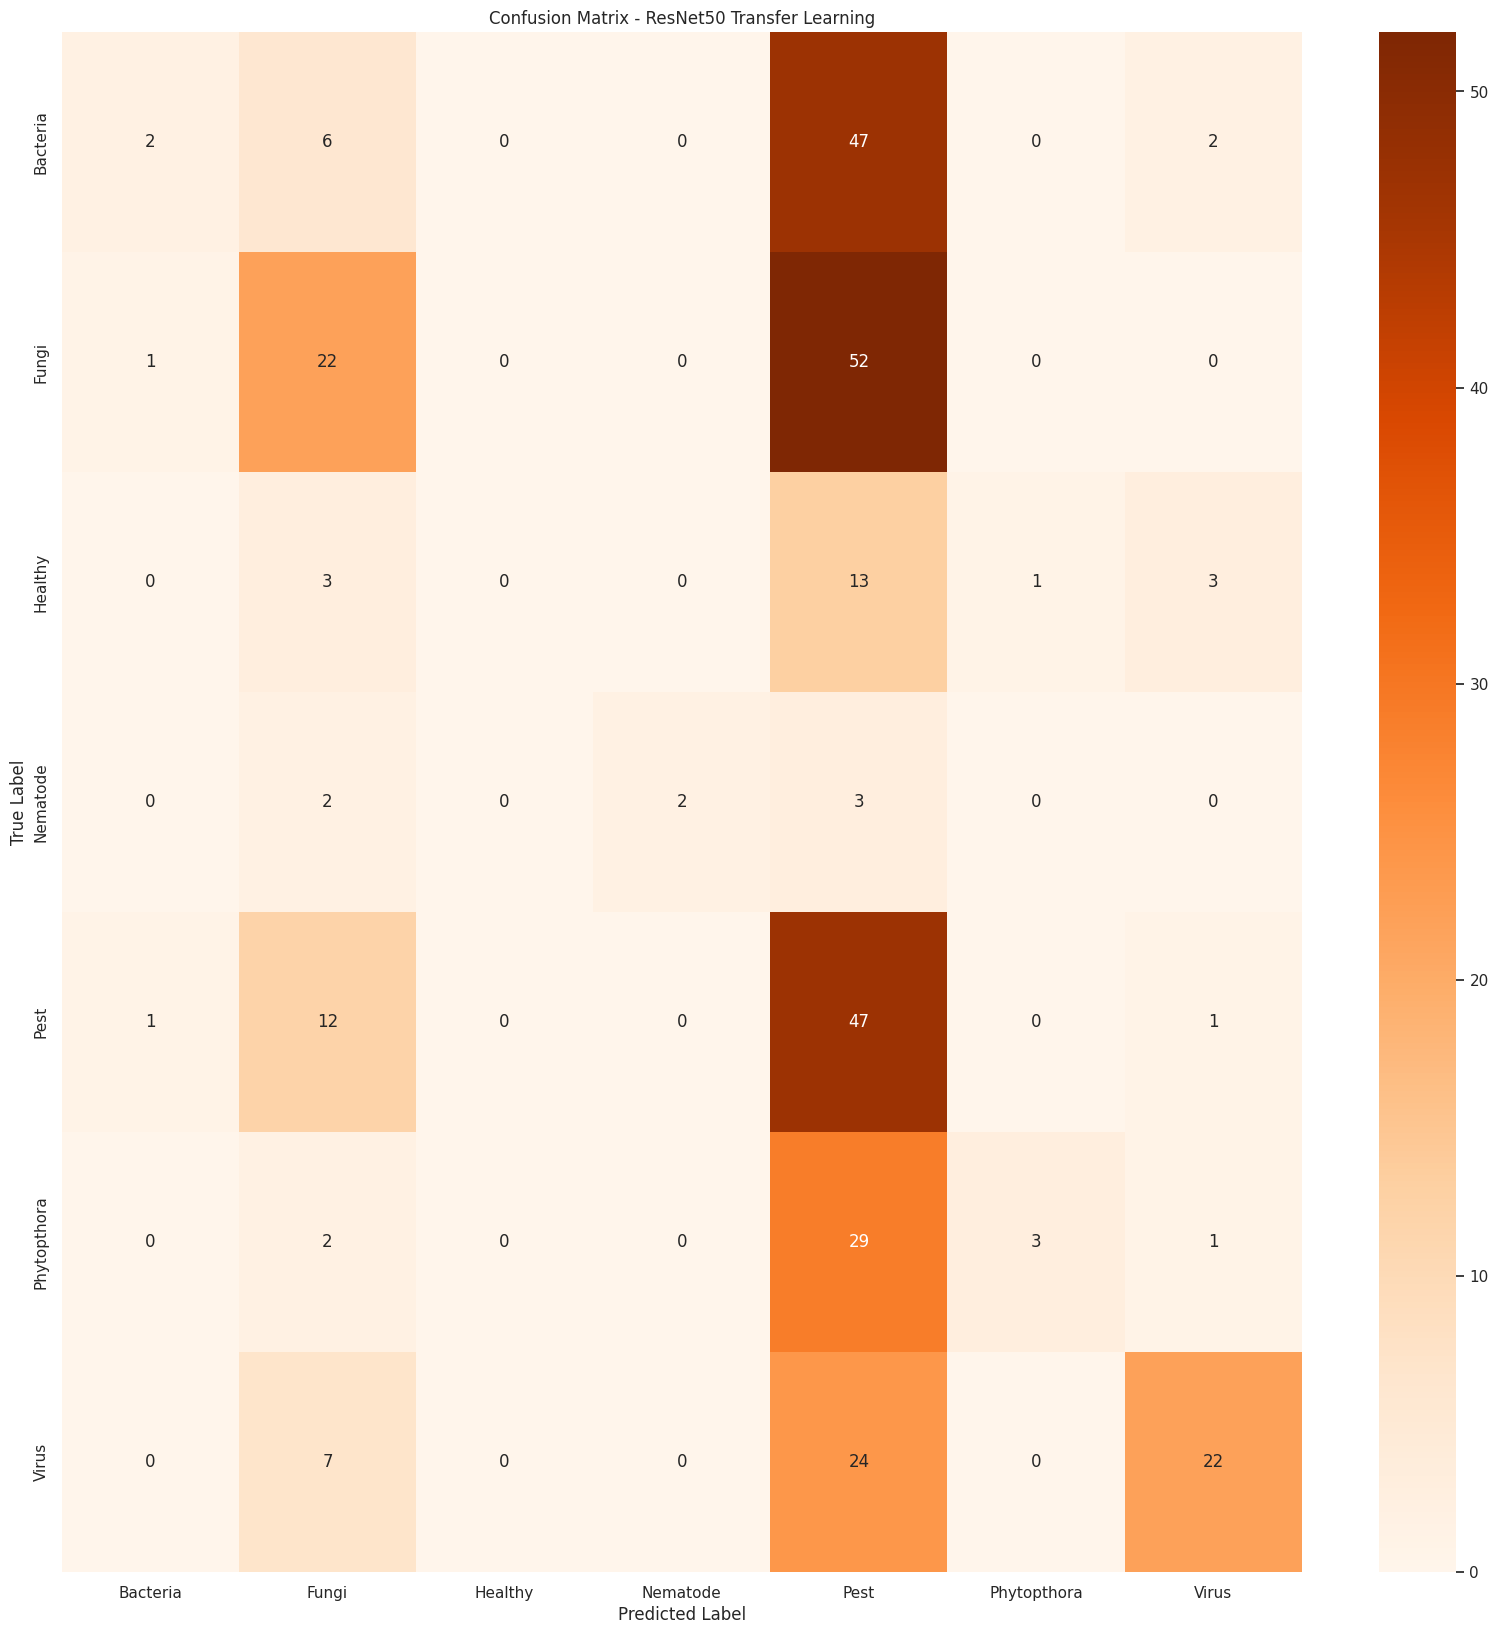
\includegraphics[width=0.75\textwidth]{image/docx_image14.png}
\caption{Confusion Matrix for ResNet50.}
\label{fig:resnet_cm}
\end{figure}

\begin{figure}[htbp]
\centering
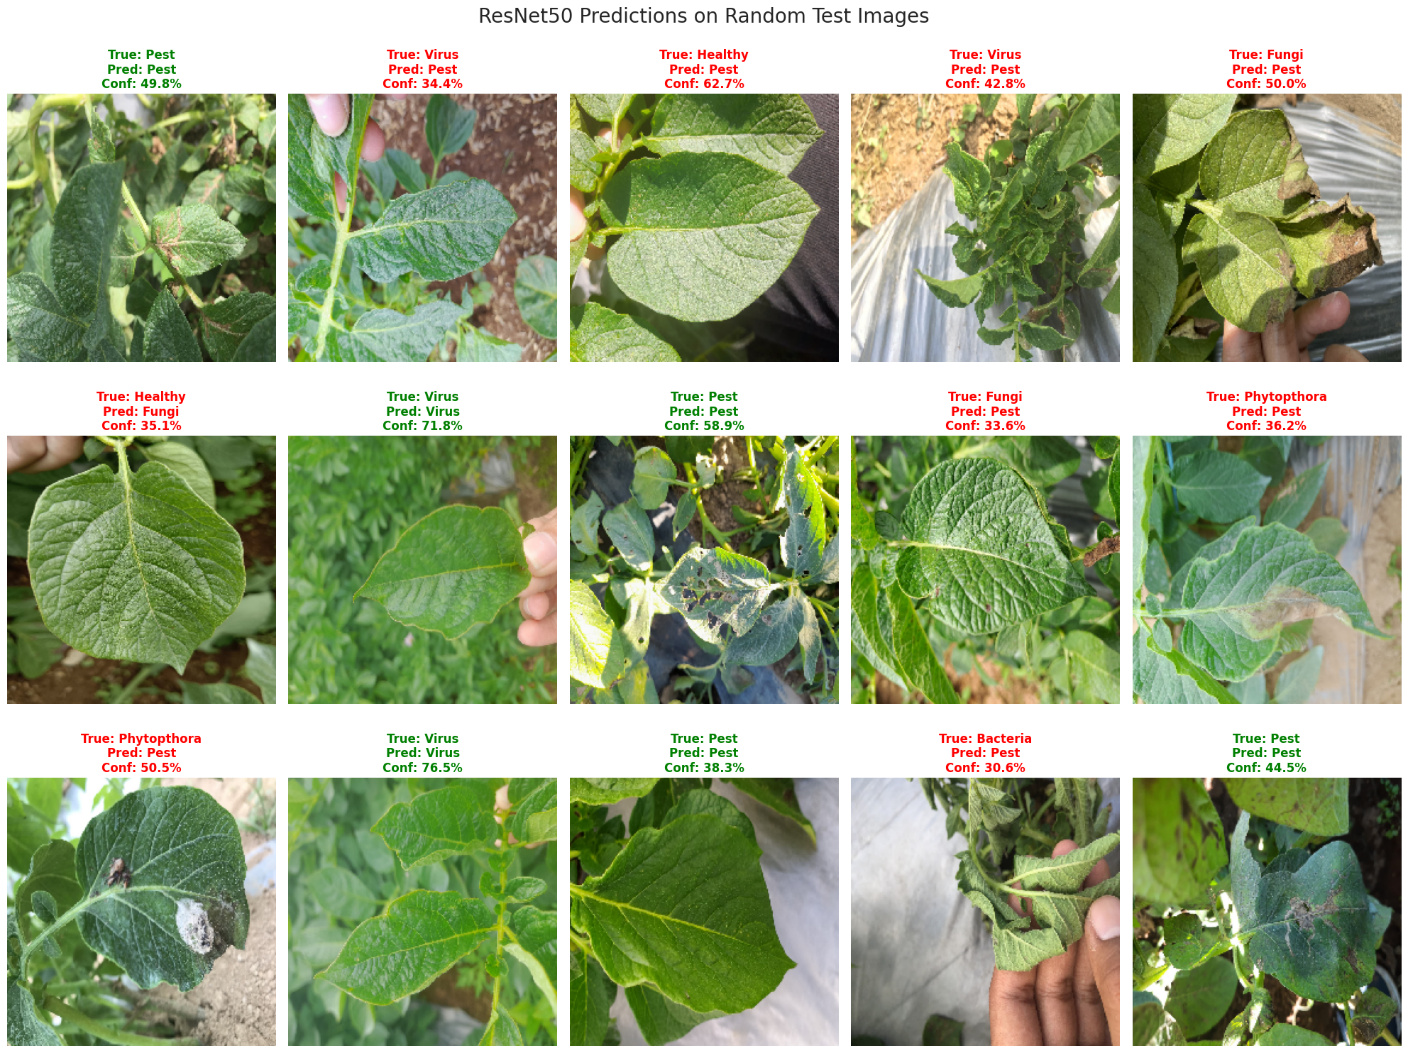
\includegraphics[width=0.9\textwidth]{image/docx_image15.png}
\caption{Random test samples classified by ResNet50.}
\label{fig:resnet_samples}
\end{figure}

\subsubsection{MobileNetV2 Results}
MobileNetV2 was set to train for 10 epochs ($\sim 370$ seconds per epoch on CPU). Early Stopping ended training after Epoch 6 and restored the Epoch 1 weights. Training accuracy rose from 30\% to 48\%, while validation accuracy remained constant at 24.35\% and validation loss rose from 1.86 to 2.01 (Figure~\ref{fig:mobilenet_curves}).

\begin{figure}[htbp]
\centering
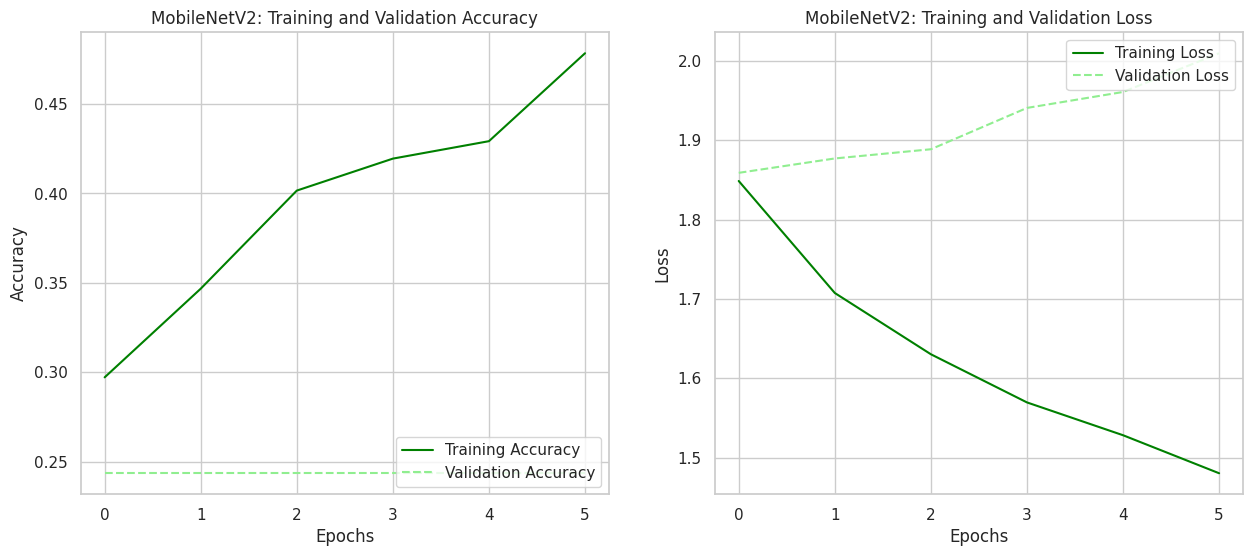
\includegraphics[width=0.9\textwidth]{image/docx_image17.png}
\caption{Training and validation learning curves for MobileNetV2.}
\label{fig:mobilenet_curves}
\end{figure}

On the test set, MobileNetV2 achieved 24.35\% accuracy and 1.8593 test loss (Table~\ref{tab:mobilenet_report}), predicting \textbf{Fungi} for all 308 test images (75 of 308, 24.35%). All other classes had 0.00 precision, recall, and F1-score, as confirmed by the confusion matrix (Figure~\ref{fig:mobilenet_cm}) and random sample predictions (Figure~\ref{fig:mobilenet_samples}), where every image received the same 27.1\% confidence for Fungi.

\begin{table}[htbp]
\caption{Summary of Classification Report (MobileNetV2)}
\label{tab:mobilenet_report}
\begin{center}
\begin{tabularx}{0.65\textwidth}{| X | c |}
\hline
\textbf{Metric} & \textbf{Score} \\
\hline
Accuracy & 24.35\% \\
\hline
Macro Avg (Precision) & 0.03 \\
\hline
Macro Avg (Recall) & 0.14 \\
\hline
Weighted Avg F1-Score & 0.10 \\
\hline
\end{tabularx}
\end{center}
\end{table}

\begin{figure}[htbp]
\centering
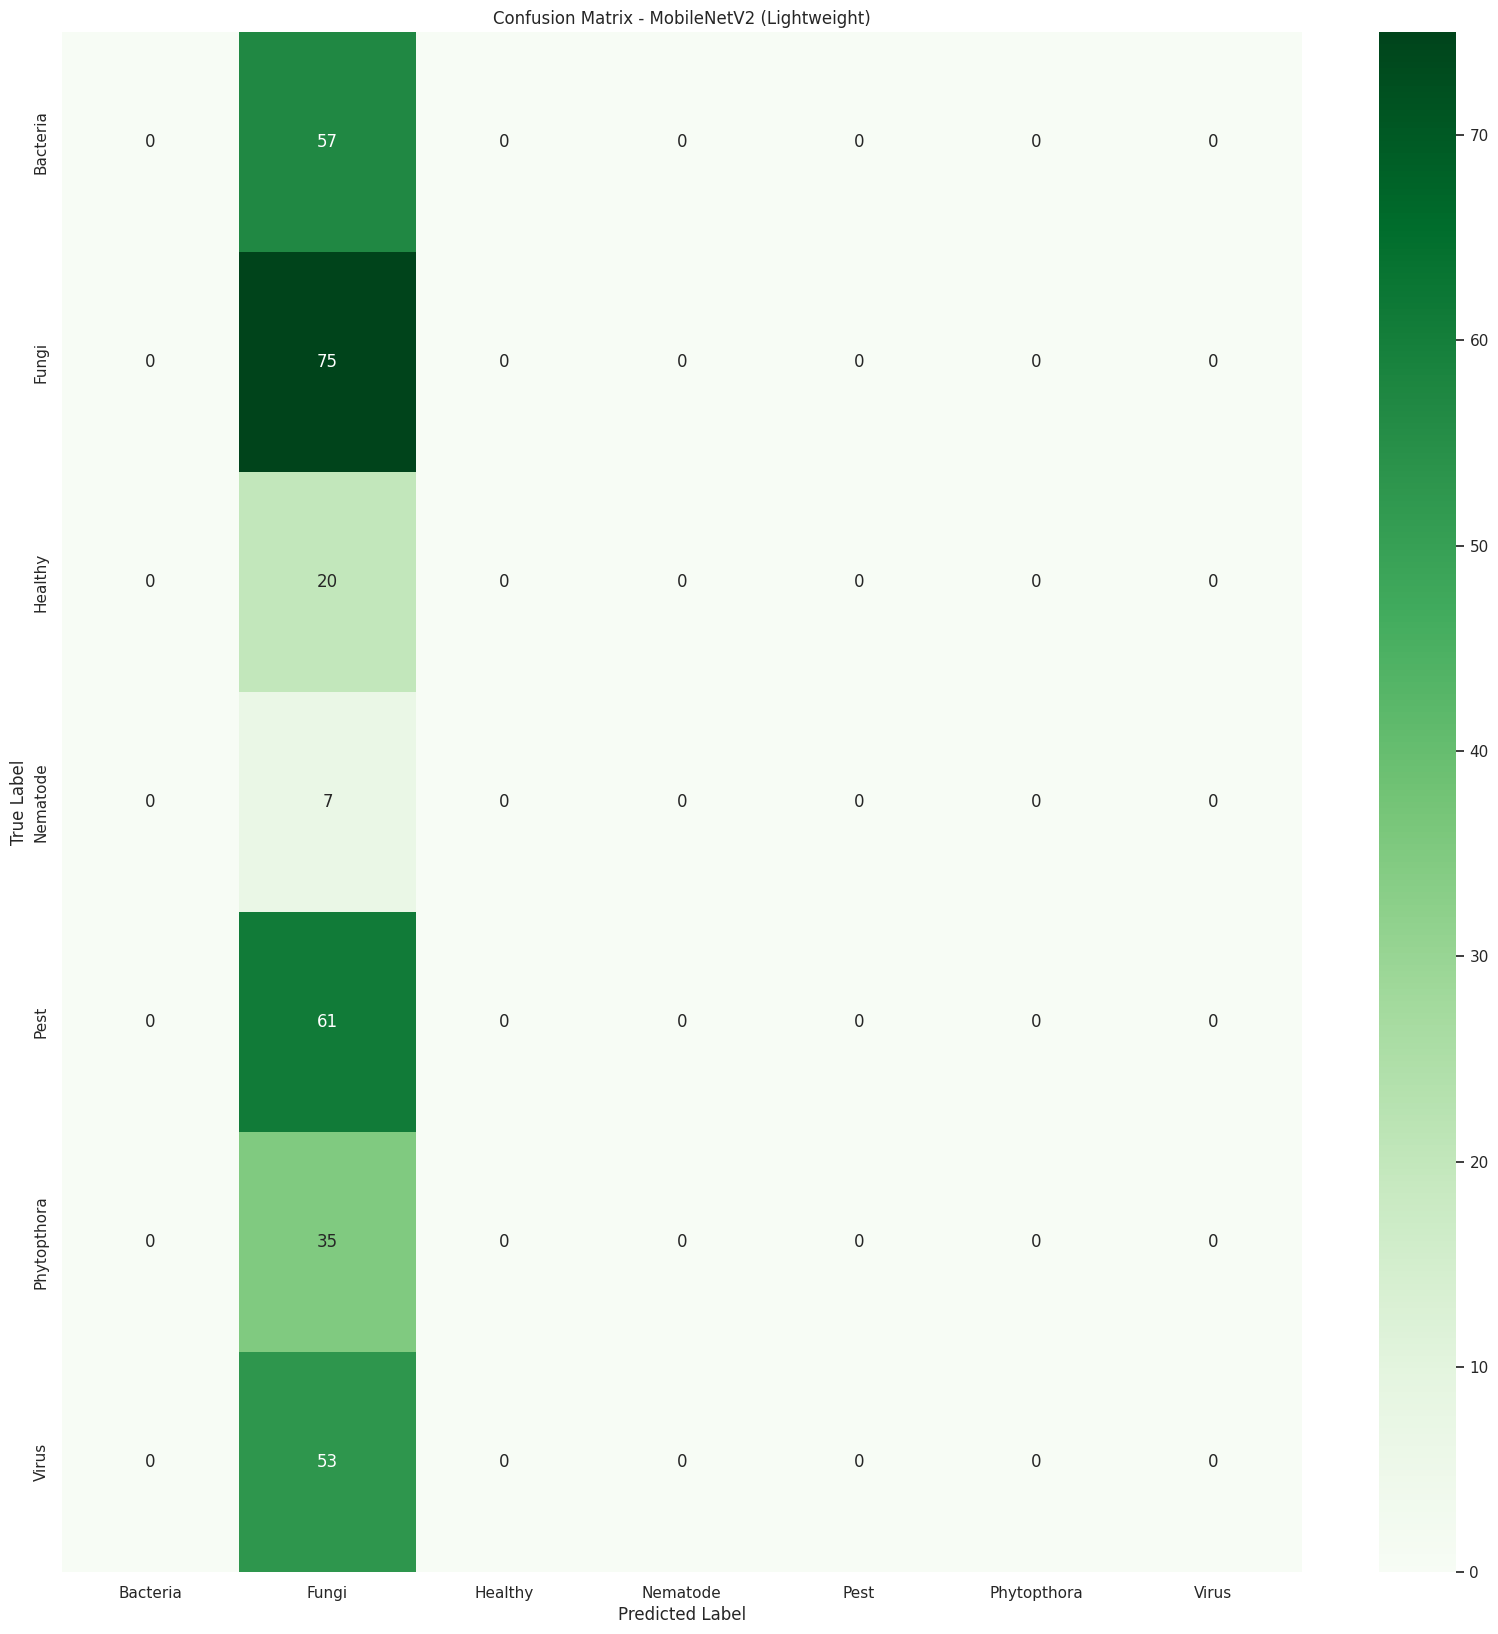
\includegraphics[width=0.75\textwidth]{image/docx_image18.png}
\caption{Confusion Matrix for MobileNetV2.}
\label{fig:mobilenet_cm}
\end{figure}

\begin{figure}[htbp]
\centering
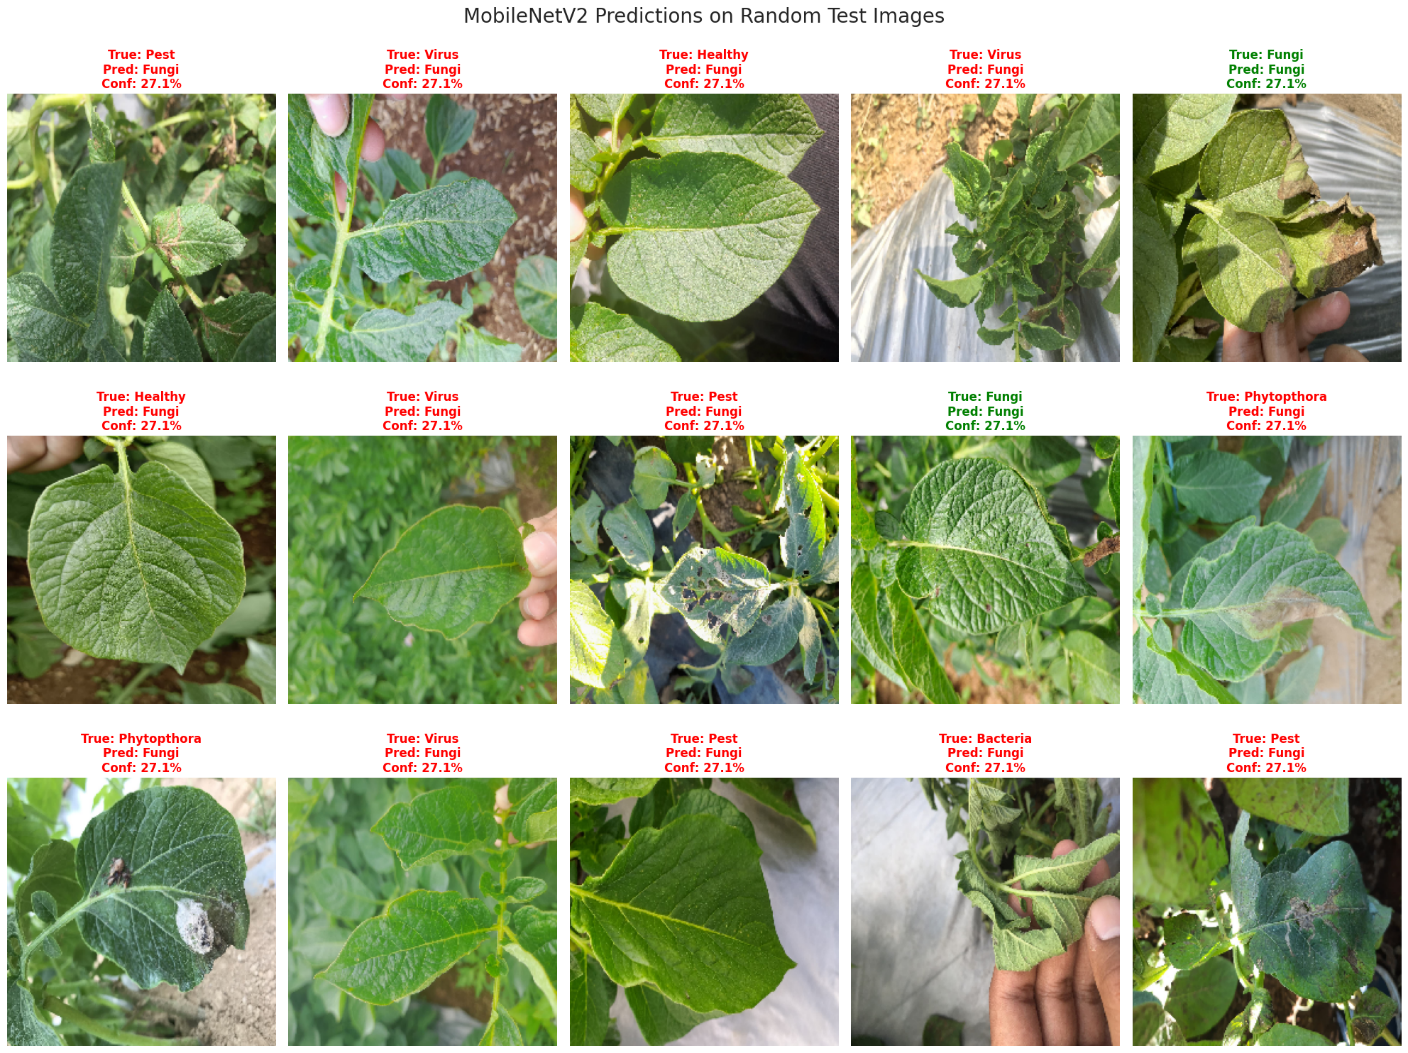
\includegraphics[width=0.9\textwidth]{image/docx_image19.png}
\caption{Random test samples predicted by MobileNetV2.}
\label{fig:mobilenet_samples}
\end{figure}

\subsection{Key Findings and Discussions}

\subsubsection{Explainable AI (XAI) Validation Results}
Grad-CAM was applied to the last convolutional layer (\texttt{conv2d\_5}) of a functional version of the Custom CNN to check whether predictions focus on leaf lesions or background noise (Figure~\ref{fig:gradcam}). Across the three sampled images (one Pest and two Fungi leaves, all predicted as Phytopthora with confidence 0.14), the heatmaps spread across borders, grid patterns, or bright background objects such as a white paper sheet.

Importantly, the notebook log shows that trained weights could not be loaded into the Grad-CAM model (\texttt{No such file or directory: best\_custom\_cnn.keras}), and the functional Grad-CAM model used a different filter configuration (32 to 256 filters) than the trained Custom CNN (16 to 128 filters). Thus, the heatmaps were produced by an untrained network, explaining the uniform 0.14 ($\approx 1/7$) confidence. The Grad-CAM pipeline works, but it must be re-run with the matching architecture and trained weights after retraining.

\begin{figure}[htbp]
\centering
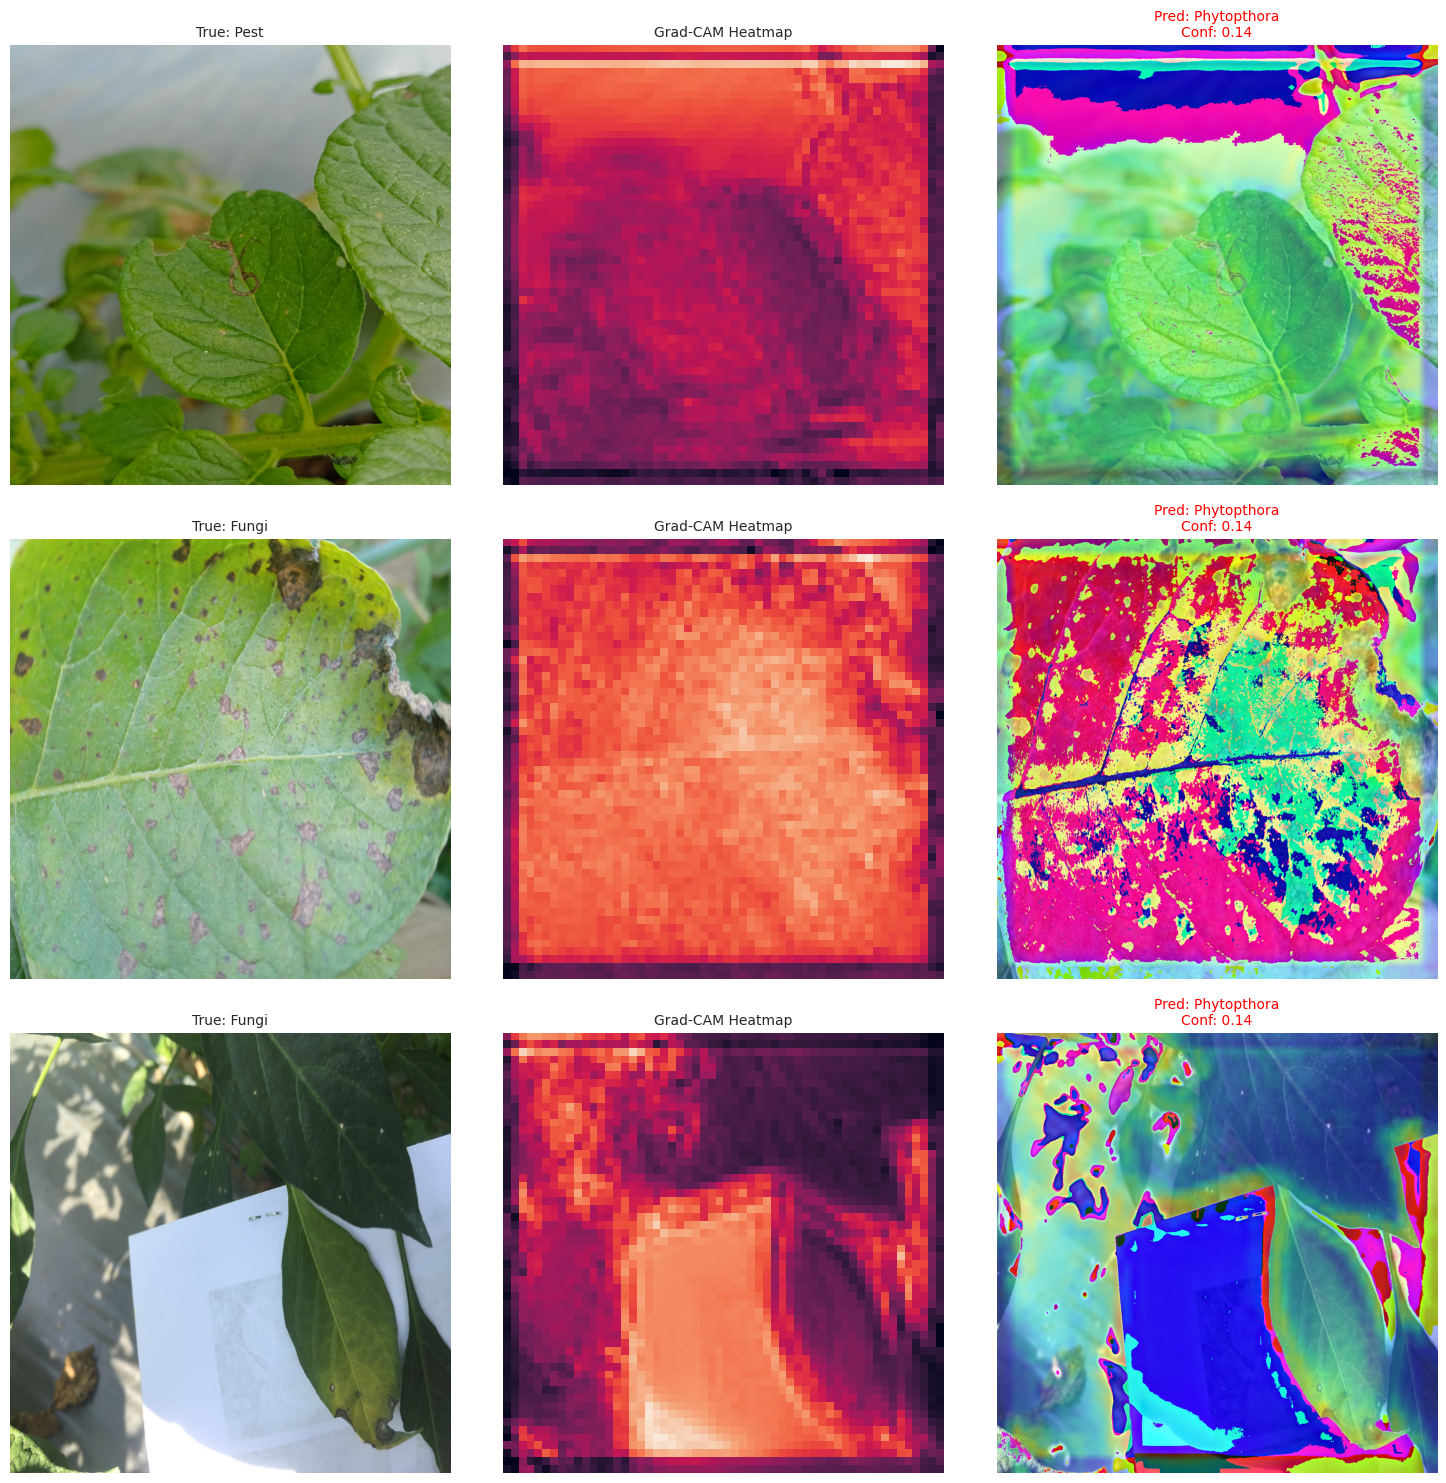
\includegraphics[width=0.9\textwidth]{image/docx_image24.png}
\caption{Grad-CAM visualizations showing the Original Image (Left), Heatmap (Center), and Superimposed Image (Right).}
\label{fig:gradcam}
\end{figure}

\subsubsection{LLM-Based Advisory Results}
The \texttt{google-genai} library was configured with a Gemini API key stored in Kaggle Secrets, and the pipeline (\texttt{get\_llm\_disease\_advice()} and \texttt{predict\_and\_explain()}, shown in Figure~\ref{fig:llm_pipeline}) was tested on a sample image from the Nematode folder. Because the saved model file was the untrained Grad-CAM network, the CNN predicted Phytopthora at 14.31\% confidence. The Gemini response correctly began with a low-confidence warning advising field inspection or consulting an agricultural extension agent, described Late Blight (\textit{Phytophthora infestans}) symptoms and favorable weather conditions, listed management and prevention steps (removing infected plants, certified seed, spacing, base watering, crop rotation), and avoided inventing pesticide doses. This demonstrates that the advisory module follows safety rules, though its diagnostic utility depends on retraining the underlying CNN.

\begin{figure}[htbp]
\centering
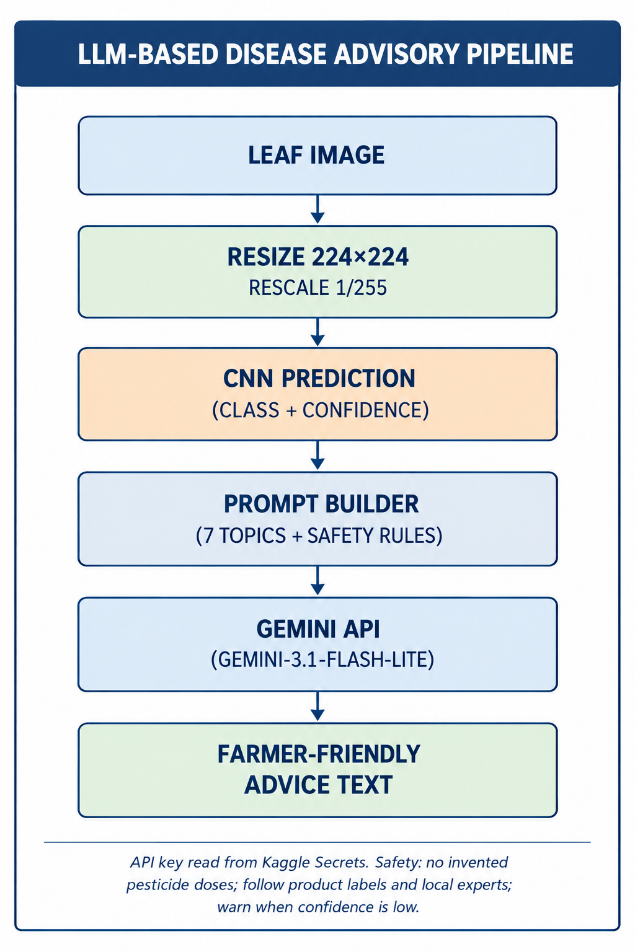
\includegraphics[width=0.9\textwidth]{image/docx_image25.png}
\caption{LLM-based disease advisory pipeline.}
\label{fig:llm_pipeline}
\end{figure}

\subsection{Comparison with State of the Art Model}
Table~\ref{tab:final_summary} summarizes the quantitative performance and efficiency metrics of the three models on the 308 unseen test images, and Figure~\ref{fig:acc_loss_comp} visualizes Test Accuracy and Test Loss. All three models remain far below the 95\% accuracy target defined in Chapter 3.

\begin{table}[htbp]
\caption{Final Performance Summary on Test Set}
\label{tab:final_summary}
\begin{center}
\begin{tabularx}{\textwidth}{| X | c | c | c | c |}
\hline
\textbf{Model} & \textbf{Test Accuracy (\%)} & \textbf{Test Loss} & \textbf{Inference Time (ms/img)} & \textbf{Model Size} \\
\hline
Custom CNN (Proposed) & 19.81\% & 1.9508 & $\sim 52.7$ ms & 1.98 MB \\
\hline
ResNet50 & 31.82\% & 1.7336 & $\sim 136.7$ ms & 92.12 MB \\
\hline
MobileNetV2 & 24.35\% & 1.8593 & $\sim 43.7$ ms & 27.21 MB \\
\hline
\end{tabularx}
\end{center}
\end{table}

\begin{figure}[htbp]
\centering
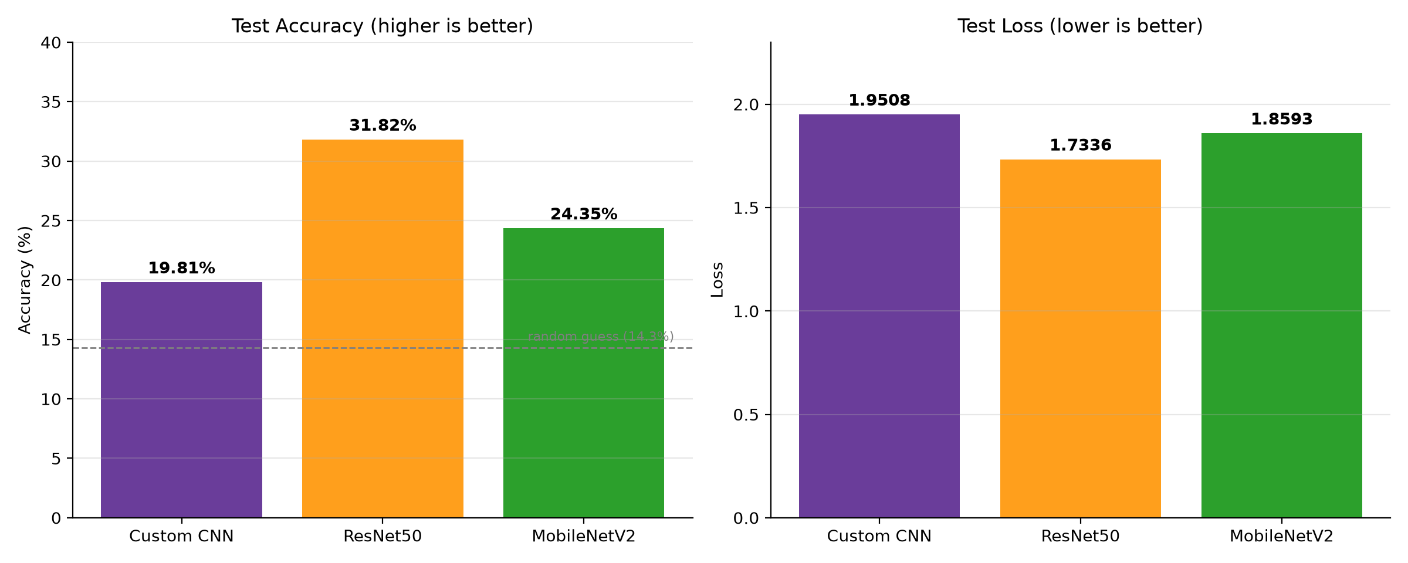
\includegraphics[width=0.85\textwidth]{image/docx_image20.png}
\caption{Comparison of Test Accuracy and Test Loss. ResNet50 has the highest accuracy and the lowest loss.}
\label{fig:acc_loss_comp}
\end{figure}

In the Radar Chart (Figure~\ref{fig:radar}), ResNet50 covers the largest area across Precision, Recall, F1-Score, and Accuracy (weighted precision 0.47). In the micro-average ROC-AUC analysis (Figure~\ref{fig:roc}), ResNet50 achieves the highest AUC ($0.7688$), followed by MobileNetV2 ($0.6652$) and the Custom CNN ($0.5889$), showing that the predicted probabilities still carry ranking signal above random chance ($0.5$). Finally, the Efficiency Trade-off plot (Figure~\ref{fig:tradeoff}) highlights that the Custom CNN is the smallest model (1.98 MB, $\sim 47\times$ smaller than ResNet50 and $\sim 14\times$ smaller than MobileNetV2) and $\sim 2.6\times$ faster than ResNet50, though retraining with GPU acceleration, ImageNet weights, more epochs, and class balancing is required for a fair accuracy comparison.

\begin{figure}[htbp]
\centering
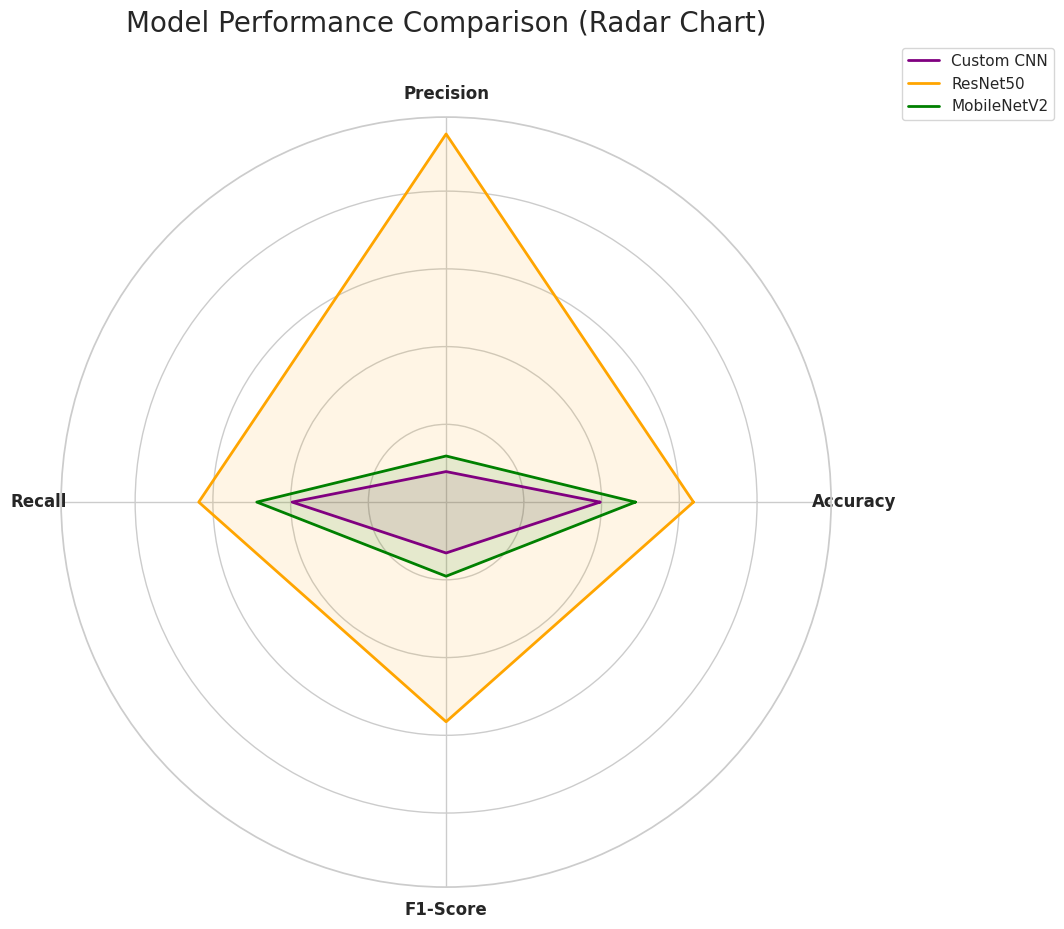
\includegraphics[width=0.75\textwidth]{image/docx_image21.png}
\caption{Radar Chart comparing Precision, Recall, F1-Score, and Accuracy.}
\label{fig:radar}
\end{figure}

\begin{figure}[htbp]
\centering
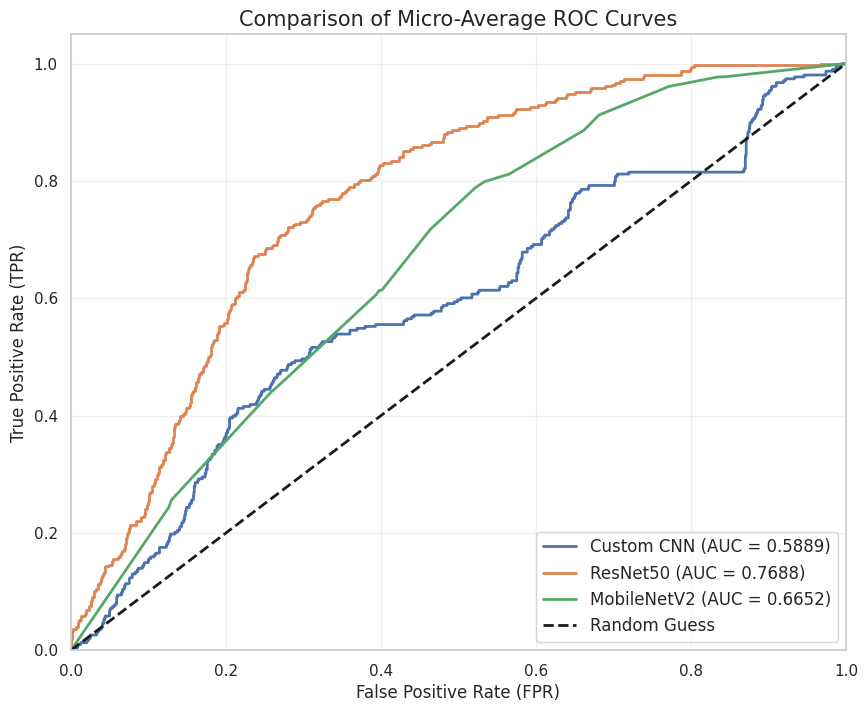
\includegraphics[width=0.8\textwidth]{image/docx_image22.png}
\caption{Micro-Average ROC Curves. ResNet50 achieves the highest AUC (0.7688).}
\label{fig:roc}
\end{figure}

\begin{figure}[htbp]
\centering
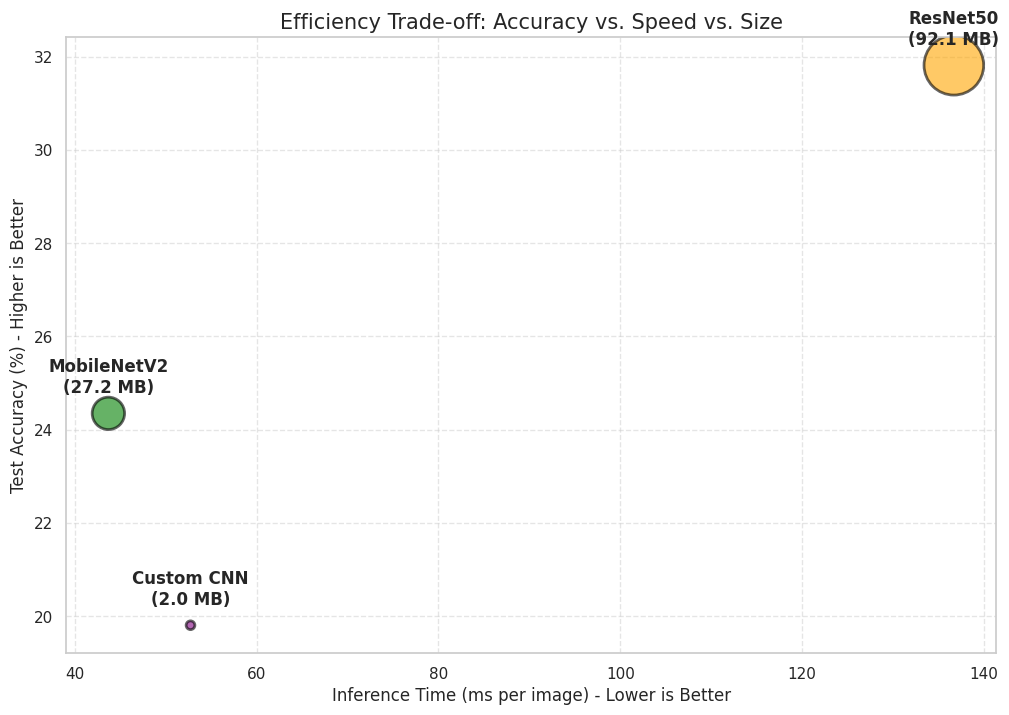
\includegraphics[width=0.85\textwidth]{image/docx_image23.png}
\caption{Efficiency Trade-off: Accuracy vs.\ Speed vs.\ Size.}
\label{fig:tradeoff}
\end{figure}

\subsection*{Summary}
This chapter presented the implementation and evaluation of the proposed system. ResNet50 achieved the highest test accuracy (31.82\%, AUC 0.7688), followed by MobileNetV2 (24.35\%) and the Custom CNN (19.81\%). While the Custom CNN is the smallest (1.98 MB) and much faster than ResNet50, both the Custom CNN and MobileNetV2 collapsed to single-class predictions under CPU-only, short-epoch training without ImageNet weights. The Grad-CAM and Gemini LLM pipelines were implemented end to end, providing a reproducible baseline ready for GPU retraining.
